\iffalse
As mentioned above one can assumed that the positron electron annihilation peak is fully suppressed.
therefore only one Gaussian peak has to be fitted together with the background function.
Additionally in the ideal case, that the majority of all \Kr\ decay events got through the LAr veto, one can expect the amplitude of the Gaussian peak to be equal to the amplitude of the not LAr veto filtered case.
The fit results in the function displayed in equation \ref{equ:FitFilters}.
\\ 

\begin{equation}
\mathrm{f}(x) = \mathrm{A}\frac{1}{\sqrt{2\pi}\mathrm{C}}\exp\left(-\frac{(x-\mathrm{B})^2}{2\mathrm{C}^2}\right) + \mathrm{D}\exp\left(\mathrm{-E}x\right) + \mathrm{F}
\label{equ:FitFilters}
\end{equation}
\\
\fi
\\


\iffalse
When looking at the not LAr veto filtered spectra we can see that over the course of the displayed energy interval no real change of the background can be seen (see figure \ref{fig:NoFilterBEGes} and \ref{fig:NoFilterCOAX}).
Theoretically however, one can expect the background count rate to behave like the phase-space function of the dominant \nuc{Ge}{76} and therefore change with energy.
So it is necessary to also consider this change in count rate over energy in the fit function.
The phase-space function of \nuc{Ge}{76} is very complex.
In this case however the energy interval is relatively small compared to the complete spectrum.
This allows the approximation that its phase-space function changes like an exponential decrease.
\fi


\iffalse
From it one can see that the overwhelming majority of the detected events were positioned close to the detectors themselves.
At longer distances, the majority of all decays were no longer measured.
This means that, while holding the simulated decay density constant, the amount of measured events should not change when enlarging the volume.
But that would also mean that the detector efficiency $\epsilon$ would have a reciprocal proportionality to the simulated volume.
Therefore, one can expect the ratio $1/ \epsilon V_{\mathrm{sim}}$ to be invariant with change of volume, provided that the volume is large enough.   
This is the reason why the usage of a smaller volume of LAr in the Monte Carlo simulation was justified.
This ratio easily be adapted to a conversion factor from the amount of measured counts in the 514keV line to the density of \Kr\ necessary to create the measured peak, just by dividing the ratio through the probability $p = 0.434\%$ of \Kr\ decaying into the excited state of \nuc{Rb}{85}.
\\
\fi












\iffalse

To be able to use this method to determine the specific activity of \Kr\ it is necessary to assume that only \Kr\ with its half life of $T_{\frac{1}{2}}$ = 10.739 yr should create a notable change in the overall count rate.
As it is necessary to suppress a jump in the count rate by the lowering of the lower energy threshold, a lower energy limit at 200 keV for the considered events must be applied.
It is also necessary to only use the data recorded by detectors that have recorded data throughout all of \gerda's active measuring times.
For this reason only the data from run 55 to 92 was used as run 53 and 54 only had a smaller amount of detectors recording.
Which detectors have ultimately used in this analysis can be seen in appendix chapter \ref.
All data used in this analysis has also been previously filtered by the standard \gerda\ analysis cuts.
\\

When finally plotting all count rates a exponential fit can be applied and from it the \Kr\ caused count rate $R_{count}(t=0)$ at the beginning of \PII\ determined.
Another Monte Carlo simulation is necessary to calculate another conversion factor 1/$\epsilon V_{sim}$.
With these two values the activity at the beginning of \PII\ can then be determined using formula \ref{equ:ActivityDieZweite}
\begin{equation}
a(t=0) = \frac{R_{\mathrm{count}}(t=0)}{\epsilon V_{\mathrm{sim}}}
\label{equ:ActivityDieZweite}
\end{equation}
\\

However, the specific \Kr\ activity determined in the previous chapter is too small as it can be expected to see any change of it in the count rate diagram.
This results from \nuc{Ar}{39} having a similar Q-value as \Kr\ having a specific activity in the order of 1 Bq/l effectively four orders of magnitude higher than \Kr\.
\nuc{Ar}{39}'S half life is with $T_{\frac{1}{2}} = 269\unit{yr}$ too long to see any change over the relatively small time window of \PII\ but it still creates a constant background so large that \Kr\ change should hardly be seen.
This leads to three possible scenarios:
\begin{enumerate}
	\item No change in count rate can be seen in the count rate plot. 
	This would any \Kr\ change would already be dominated by the statistical variations of radioactive isotopes with a much higher half life.
	%In this case only an upper limit on \Kr\ specific activity can be determined as it has to be smaller than the error of the count rates in the diagram.
	\item A change can be seen in the count rate and \Kr\ is responsible for this change with a count rate much higher than expected from the previous chapter.
	This result can be used falsify the results determined in chapter \ref{sec:SAfrom514}.
	\item A change can be seen in the count rate but \Kr\ is not responsible but rather another radioactive isotope with a similar half life whoes specific activity has been expected to be too low to be measured.
	
\end{enumerate}
This means that in the case a notable change can be detected it has to be determined whether it originates from the \Kr\ or \nuc{Ar}{42}.
This can be done be applying two exponential fit functions through the count rate diagram each fixed to the half life of the respective isotope and determining which fit has the better goodness using a chi-squared test.
\\

\section{Monte Carlo}

However, before the count rate plot will be produced it is of interest to find out what count rate can be expected from the \Kr\ when assuming the resulting from the specific activity of the first method present.
This can be calculated using the aforementioned conversion factor determined in the Monte Carlo simulation.
The difference between this simulation in the one calculated in the previous chapter is that this time the actual \Kr\ decays will be simulated instead only the 514 keV gamma emissions.
It can be expected, however, that the detector efficiency determined from this simulation will be much smaller than previously as only a minority of beta electrons emitted from the decays are expected to create a measurable event.
This is due to the much shorter range of electrons in the LAr as well as their lower transmission factor in the germanium leaving many electrons to be captured in the dead layer of the detectors.
For this reason a much higher amount of N = 1 billion \Kr\ decays in a volume of again $V_{sim} = 17.65 \mathrm{m}^3$ were simulated.
\\

Figure \ref{fig:Sim1Spektrum} shows the simulated energy spectrum of all measured events in the detectors considered.
On can see that the 514 keV gamma peak contains a relativity high number fo counts being caused by only 0.434$\%$ of all \Kr\ decays.
This suggests that the majority of measured events at energy lower than 514 keV must have been caused by the gammas.
When comparing the number of events in the investigated energy range of 200 to 400 keV divided by the line counts of the 514 keV peaks of the spectra \ref{fig:Sim1Spektrum} and \ref{fig:PhasenraumMC514} one is able to determine that only 20.1$\%$ of all events in this energy interval have been caused by beta electrons.
Since the dead layer of the Monte Carlo simulation is only an approximation to the real dead layer, a small systematic error is generated. 
However, since only a small number of events were caused by beta electrons, for which the dead layer is important, this error can be neglected. 
\\

In the colored area of figure \ref{fig:Sim1Spektrum} a number of $\Delta N =$ 1438 counts.
This results in a detector efficiency of 
\begin{equation*}
\epsilon = \frac{\Delta N}{N_{sim}} = (1.438 \pm 0.038) \times 10^{-6} \frac{\unit{cts}}{\unit{decay}}
\end{equation*}
If you again take its reciprocal value and divide it by the volume in which the decays occurred, you get the volume-independent conversion factor from the measured amount of counts to the decay density necessary to create this amount.
\begin{equation*}
\frac{1}{\epsilon V_{sim}} = (39.39 \pm 1.04) \frac{\unit{decay}}{\unit{cts \times l}}
\end{equation*}
In this case it can again be assumed that this value is volume-independent, since the same volume was used as in the first simulation and the beta electrons are supposed to have an even shorter range than the gamma.
This is why most decays that generate a signal must also have occurred in the immediate vicinity of the detectors.
\\

To now calculate the expected count rate of \Kr\ with the specific activity of the first method ($\bar{a} = (0.508\pm0.086)\frac{\unit{mBq}}{\unit{l}}$), the specific activity has to be divided by the conversion factor resulting in a count rate of 
\begin{equation*}
R_{\mathrm{M1}} = \bar{a} \times V_{\mathrm{sim}} \epsilon =  (1.29\pm0.25) \times 10^{-5} \frac{\unit{cts}}{\unit{s}}
\end{equation*}
in the energy range of 200 to 400 keV.

\begin{figure}
	\centering
	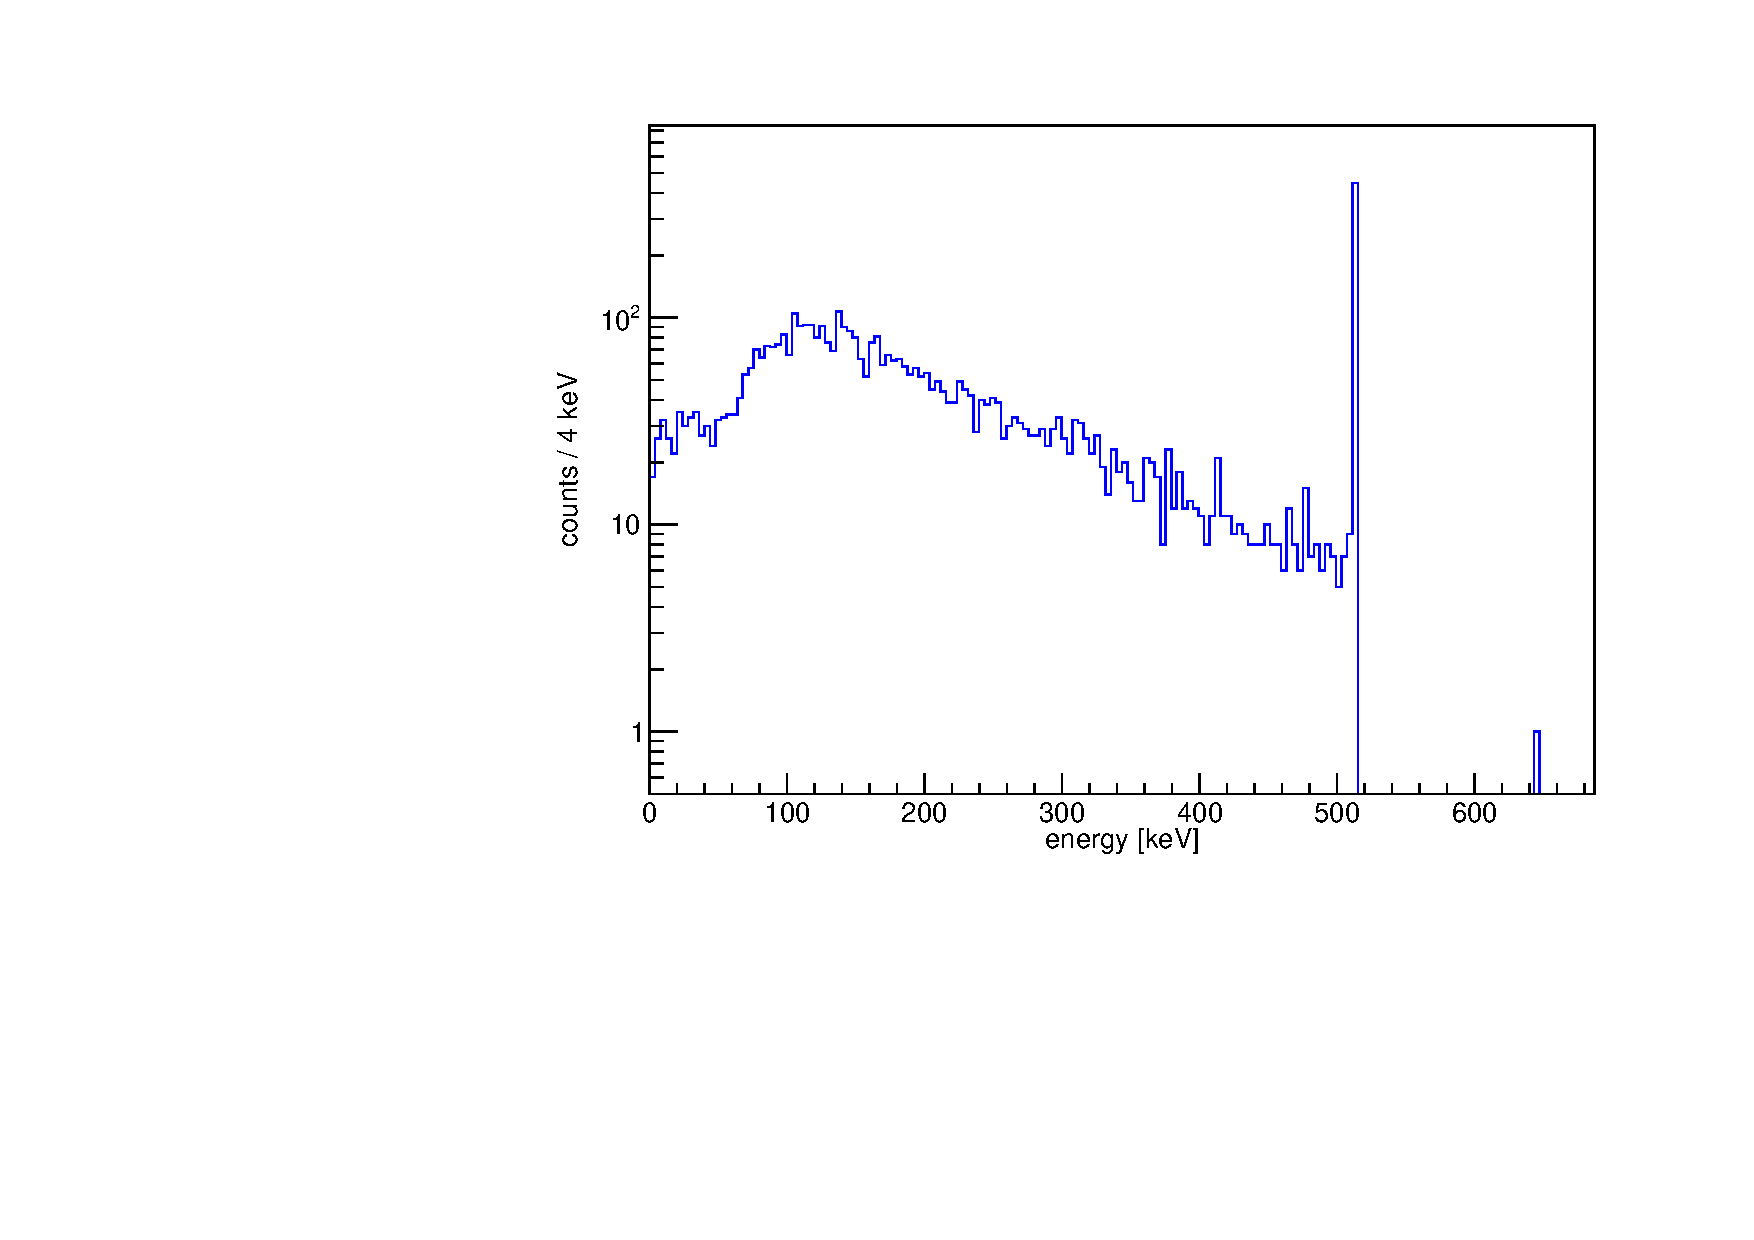
\includegraphics[width=0.6\textwidth]{./Bilder/Sim1Phasenraum.pdf}
	\caption{
		Energy spectrum computed by simulating 1 billion \Kr\ decays and plotting the counts of events by their corresponding energy.
		The blue colored area represents the amount of counts used for the calculation of the detector efficiency.
		From it can be seen, that the majority of events were created by the photons of the 514 keV peak and only about 20$\%$ from the electrons of every other \Kr\ decay.
	}
	\label{fig:Sim1Spektrum}
\end{figure}

\section{Count rate}

As explained above for the determination of the count rate diagram only those events are considered that lie in the interval of the energy limits and have been measured in one of those detectors that was always recording in \gerda's active measuring time. 
All remaining events were now plotted in figure \ref{fig:ZeitLimits} displaying the amount of measured counts per week over the remaining portion of \PII.
\\

Due to the \gerda\ setup not always continuously measuring one has to determine the actual lifetime fractions of the detectors in the respective weeks.
For this the test pulse signal can be used again.
When plotting all measured test pulse events in a diagram similar to \ref{fig:ZeitLimits} multiplying each bar by 20 s one results in the actual measuring times in each week.
By also dividing each bin by the amount of one week one results in the lifetime fraction diagram as seen in figure \ref{fig:livetime}.
\\

The count rate diagram can now finally be obtained by dividing the bins of the count diagram through the measuring times of the respective weeks.
The resulting diagram can be seen in figure \ref{fig:ChangeInEventRate}.

\begin{figure}[t!]
	\centering
	\begin{minipage}[t]{.475\textwidth}
		\centering
		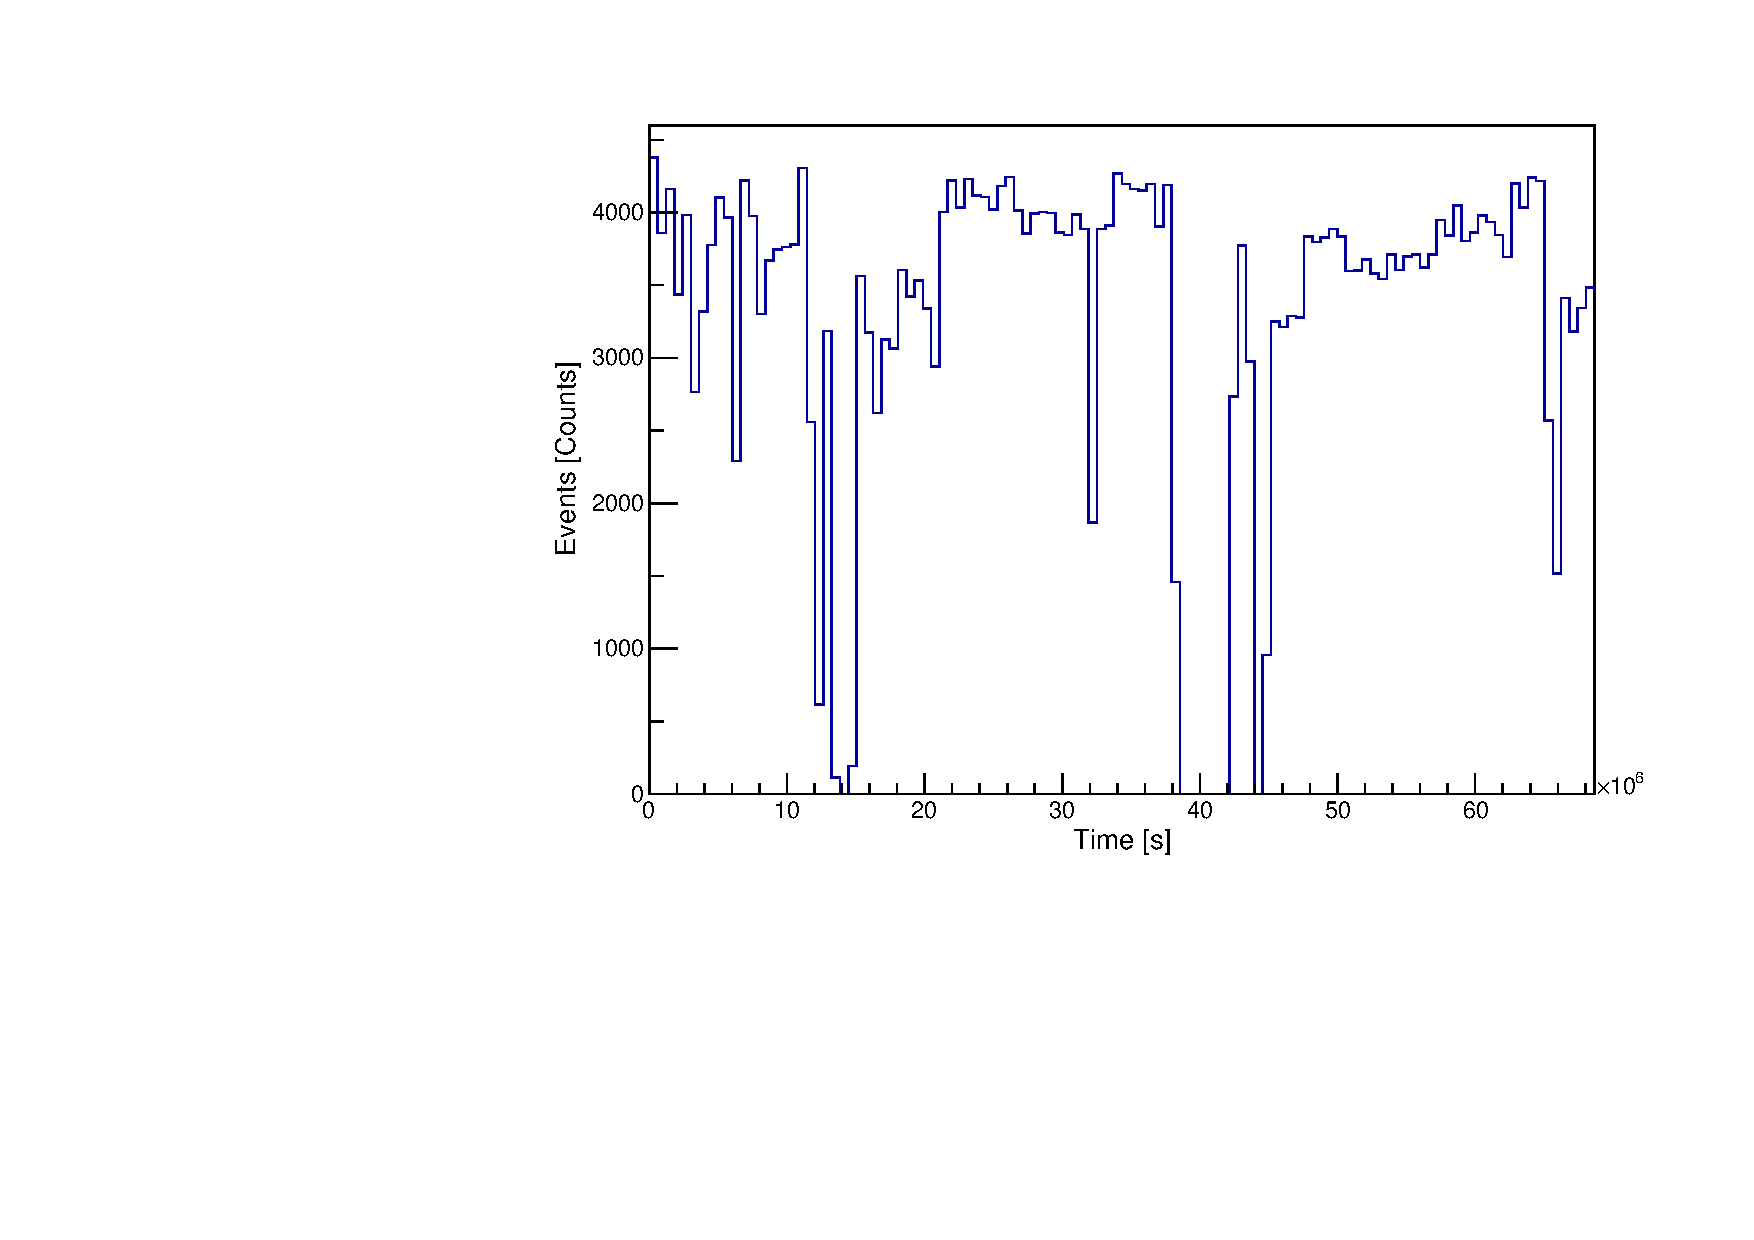
\includegraphics[width=\textwidth]{./Bilder/ZeitverlaufLimits.pdf}
		\caption{energies between 200 and 400 keV}
		\label{fig:ZeitLimits}
	\end{minipage}\hfill%
	
	\begin{minipage}[t]{.475\textwidth}
		\centering
		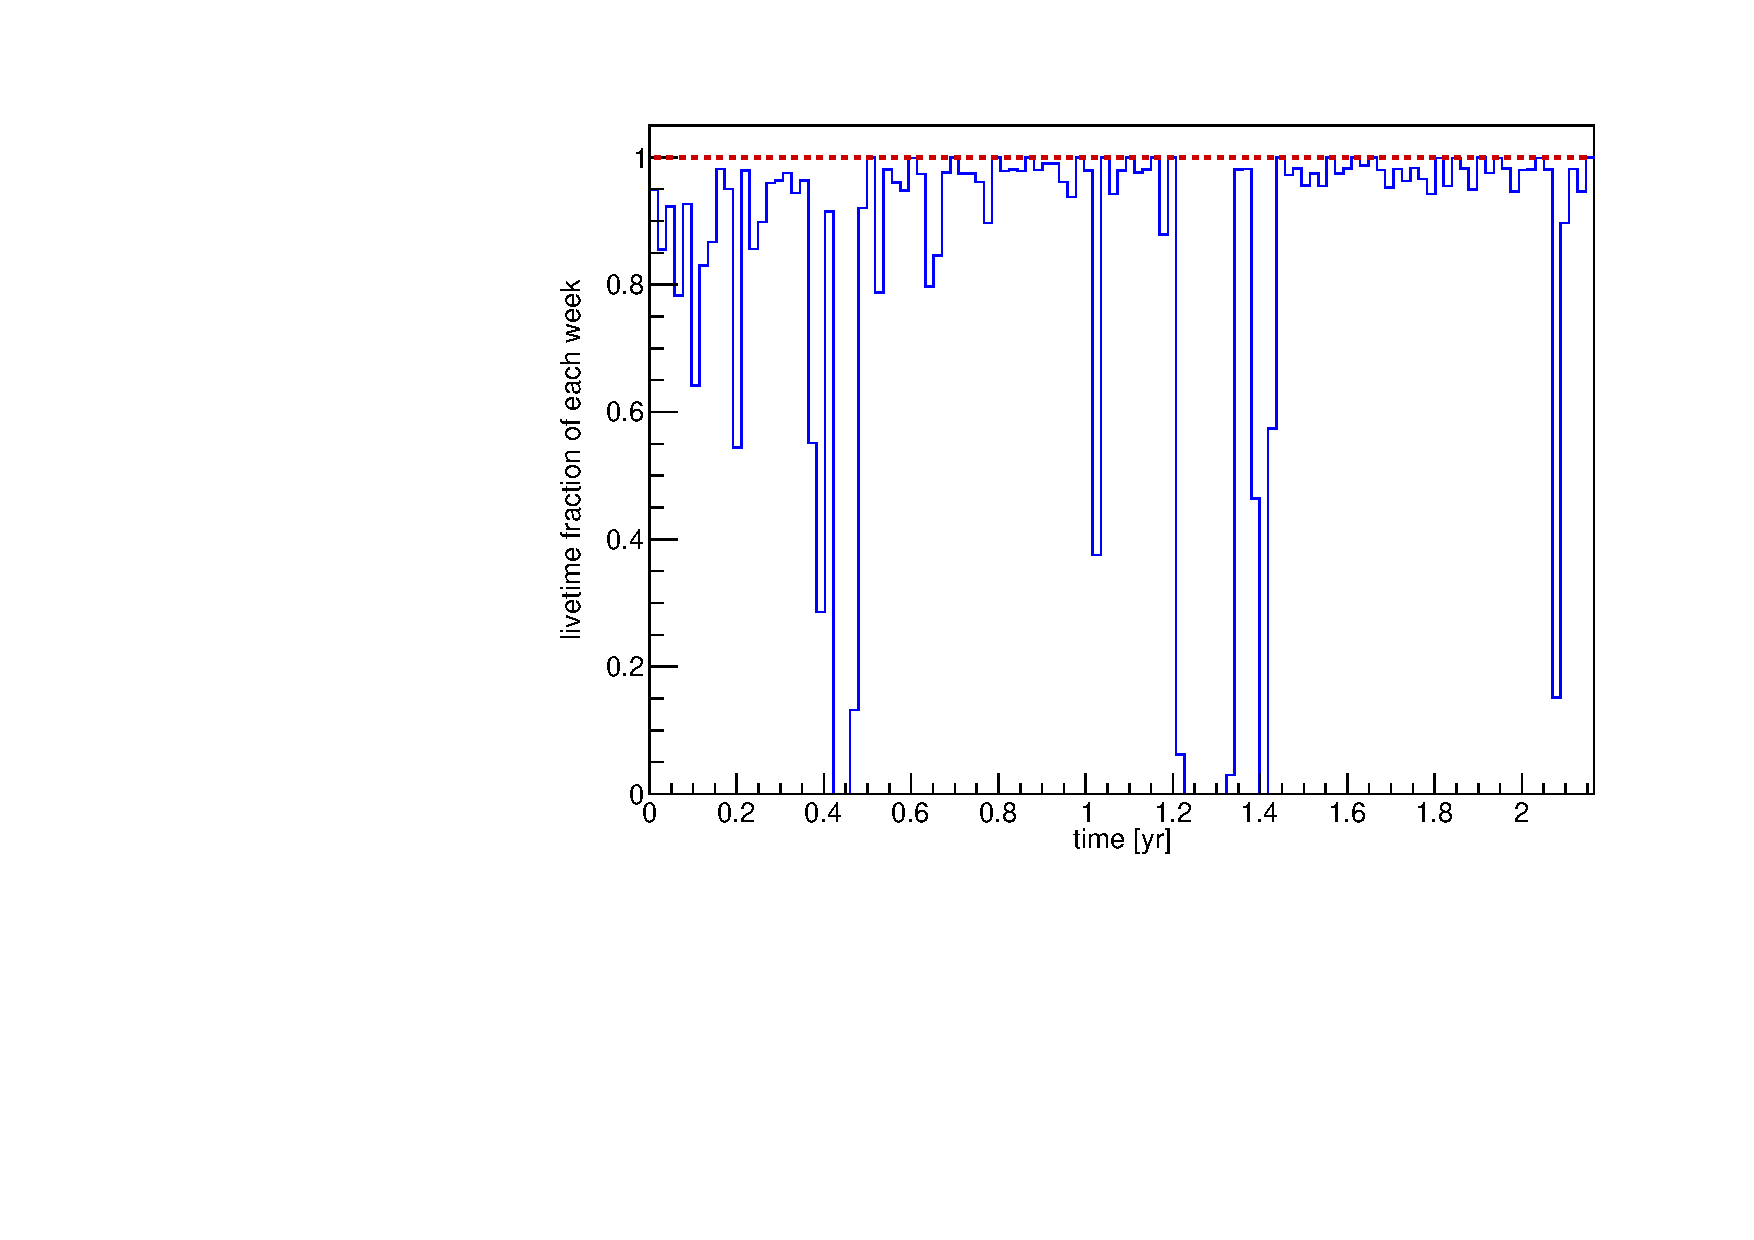
\includegraphics[width=\textwidth]{./Bilder/onceInALivetime.pdf}
		\caption{}
		
		\label{fig:livetime}
	\end{minipage}\hfill%
\end{figure}

\begin{figure}
	\centering
	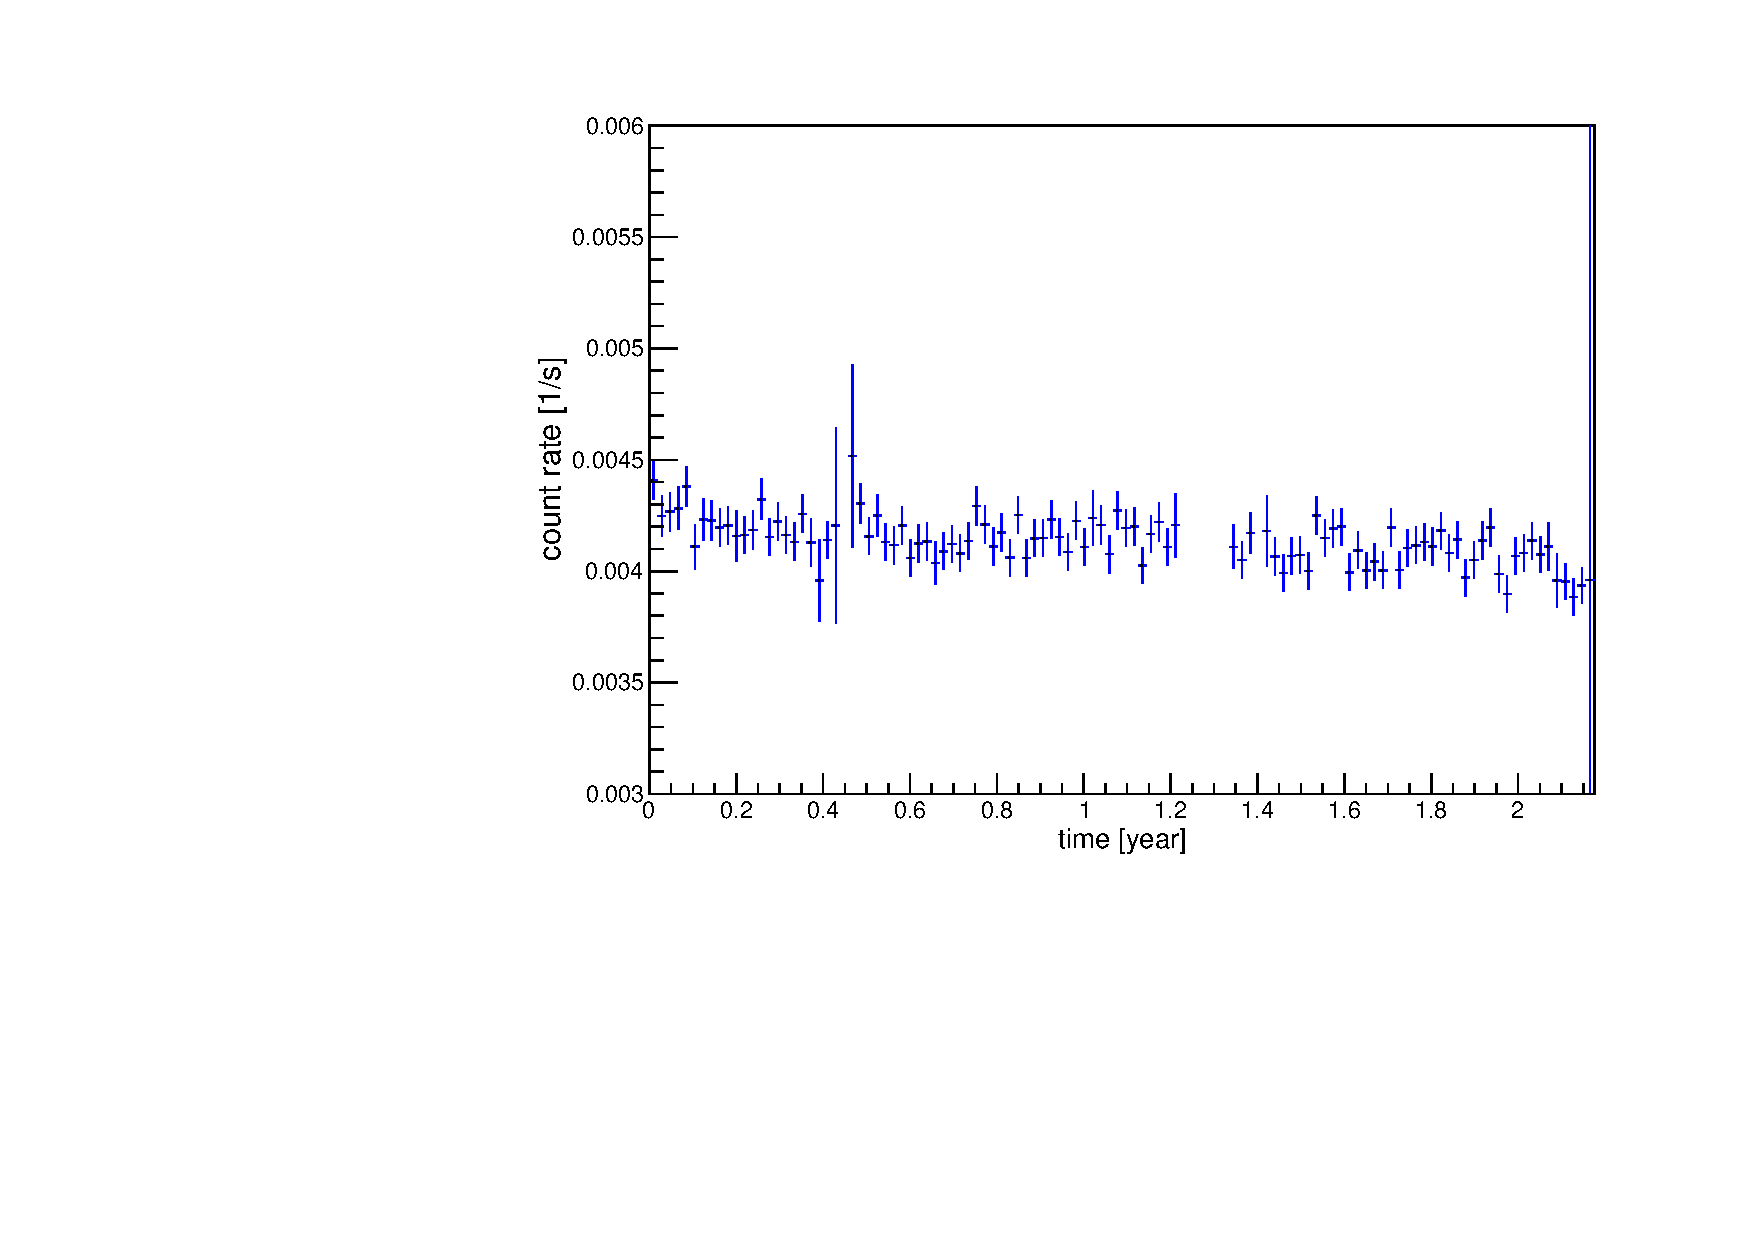
\includegraphics[width=0.6\textwidth]{./Bilder/eventRate.pdf}
	\caption{
		Count rate of measured events between 200 and 400 keV over the course of \PII.
		A continuous change in rate can be seen. 
		One can now apply a fit using function \ref{equ:FitFilters2} and through it determine the count rate of \Kr\ at the start of \PII.
	}
	\label{fig:ChangeInEventRate}
\end{figure}

As you can see, the scale of the count rate over the entire coarse one of \PII\ is in the order of 10$^{-3}$, which means that one should hardly see the count rate of \Kr\ determined from Monte Carlo, since it is two orders of magnitude smaller.
Even the errors of the measured values in the graph have a value an order of magnitude bigger, which is why it should not be visible at all.
\\

However, when fitting this plot with fit function 
\begin{equation}
\mathrm{f}(x) = \mathrm{A}\times\exp\left(-\frac{\log(2)}{\mathrm{B}} x \right) + \mathrm{C}
\label{equ:FitFilters2}
\end{equation}
with B fixed as \Kr's half life of 10.739yr, one can see from the resulting fitting plot in figure \ref{fig:eventRateFit} that a notable change in time can actually be detected.
With Fit parameter A$ = (1.495\pm0.227) \times 10^{-3}\frac{\unit{cts}}{\unit{s}}$, which corresponds to the count rate of \Kr\ at the beginning of \PII\, and the conversion factor $1/\epsilon V_{\mathrm{sim}}$ determined in the Monte Carlo simulation, the specific \Kr\ activity can be calculated using the formula \ref{equ:ActivityDieZweite}.
This results in a value of
\begin{equation*}
a(t = 0) = (58.89\pm10.50) \frac{\unit{mBq}}{\unit{l}}
\end{equation*}
which would be two orders of magnitude higher than the value determined from the first method.
But whether or not one can use this value to make any form of statement about \Kr's specific activity  depends on how well one could also apply an exponential fit function using \nuc{Ar}{42}'s half life through the data points.
\\

Figure \ref{fig:Argon} shows the resulting fitting plot of an \nuc{Ar}{42} decay also using function \ref{equ:FitFilters2}.
\\

Both of these fit functions have results far to big for what was actually expected from them.
In the case of the \nuc{Ar}{42} fit results only $10^{-4}$ cts/s would be attributed to \nuc{Ar}{39} whereas this isotope was expected to be the major source of count rate in this interval with its specific activity much higher then \Kr\ and \nuc{Ar}{42}.
However, one can see that the chi-squared $\chi^2$ values of the two exponential fit functions show that they do equally well in fitting the presented data.
This is probably mainly due to the fact that only a relatively short time was measured compared to the half-lives of the two isotopes.
Which isotope is responsible for the change in the count rate cannot be determined with the values measured so far.
Unfortunately, it can be concluded that this approach makes no statement about the specific activity of \Kr\.



\begin{figure}[t!]
	\centering
	\begin{minipage}[t]{.475\textwidth}
		\centering
		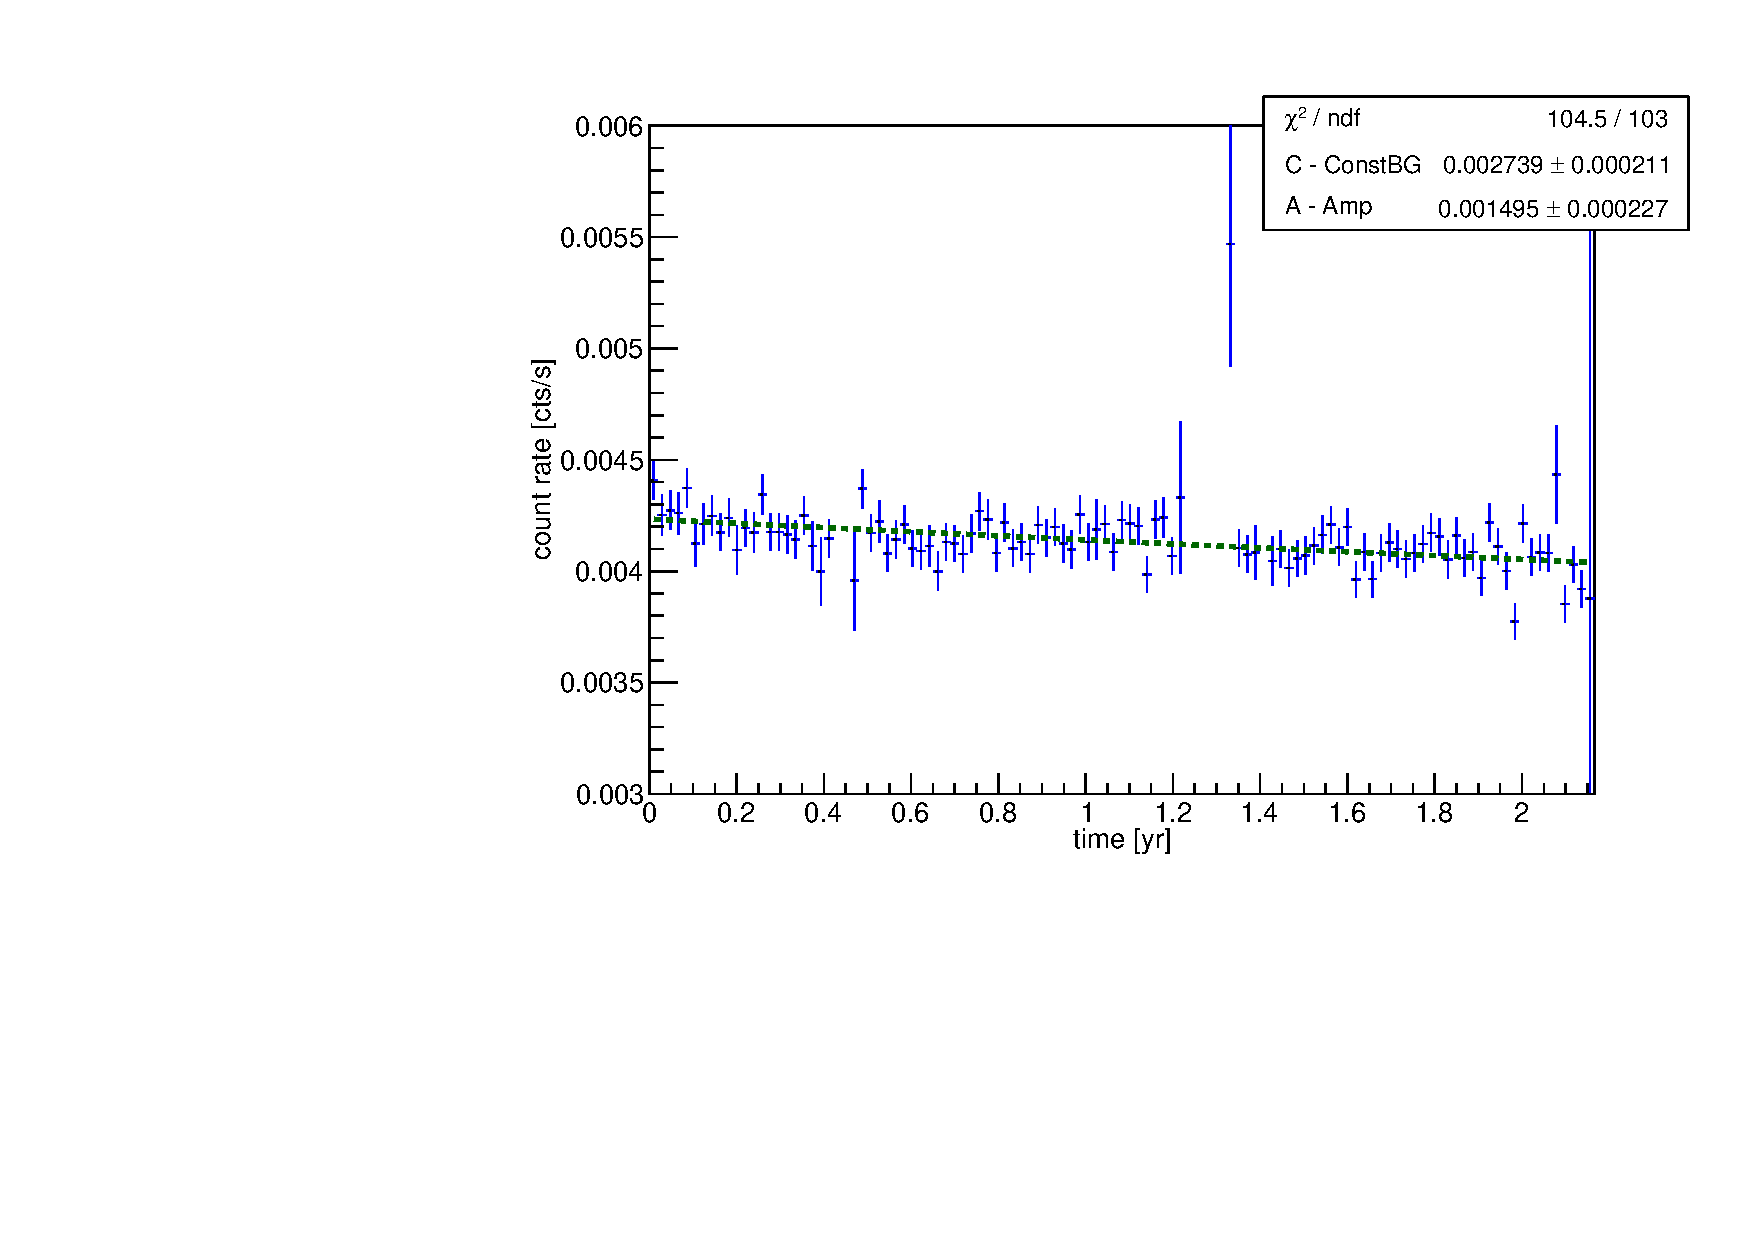
\includegraphics[width=\textwidth]{./Bilder/eventRateFit.pdf}
		\caption{
			Energy spectrum computed by simulating 1 billion \Kr\ decays and plotting the counts of events by their corresponding energy.
			The blue colored area represents the amount of counts used for the calculation of the detector efficiency.
			From it can be seen, that the majority of events were created by the photons of the 514 keV peak and only about 20$\%$ from the electrons of every other \Kr\ decay.
		}
		\label{fig:eventRateFit}
	\end{minipage}\hfill%
	\begin{minipage}[t]{.475\textwidth}
		\centering
		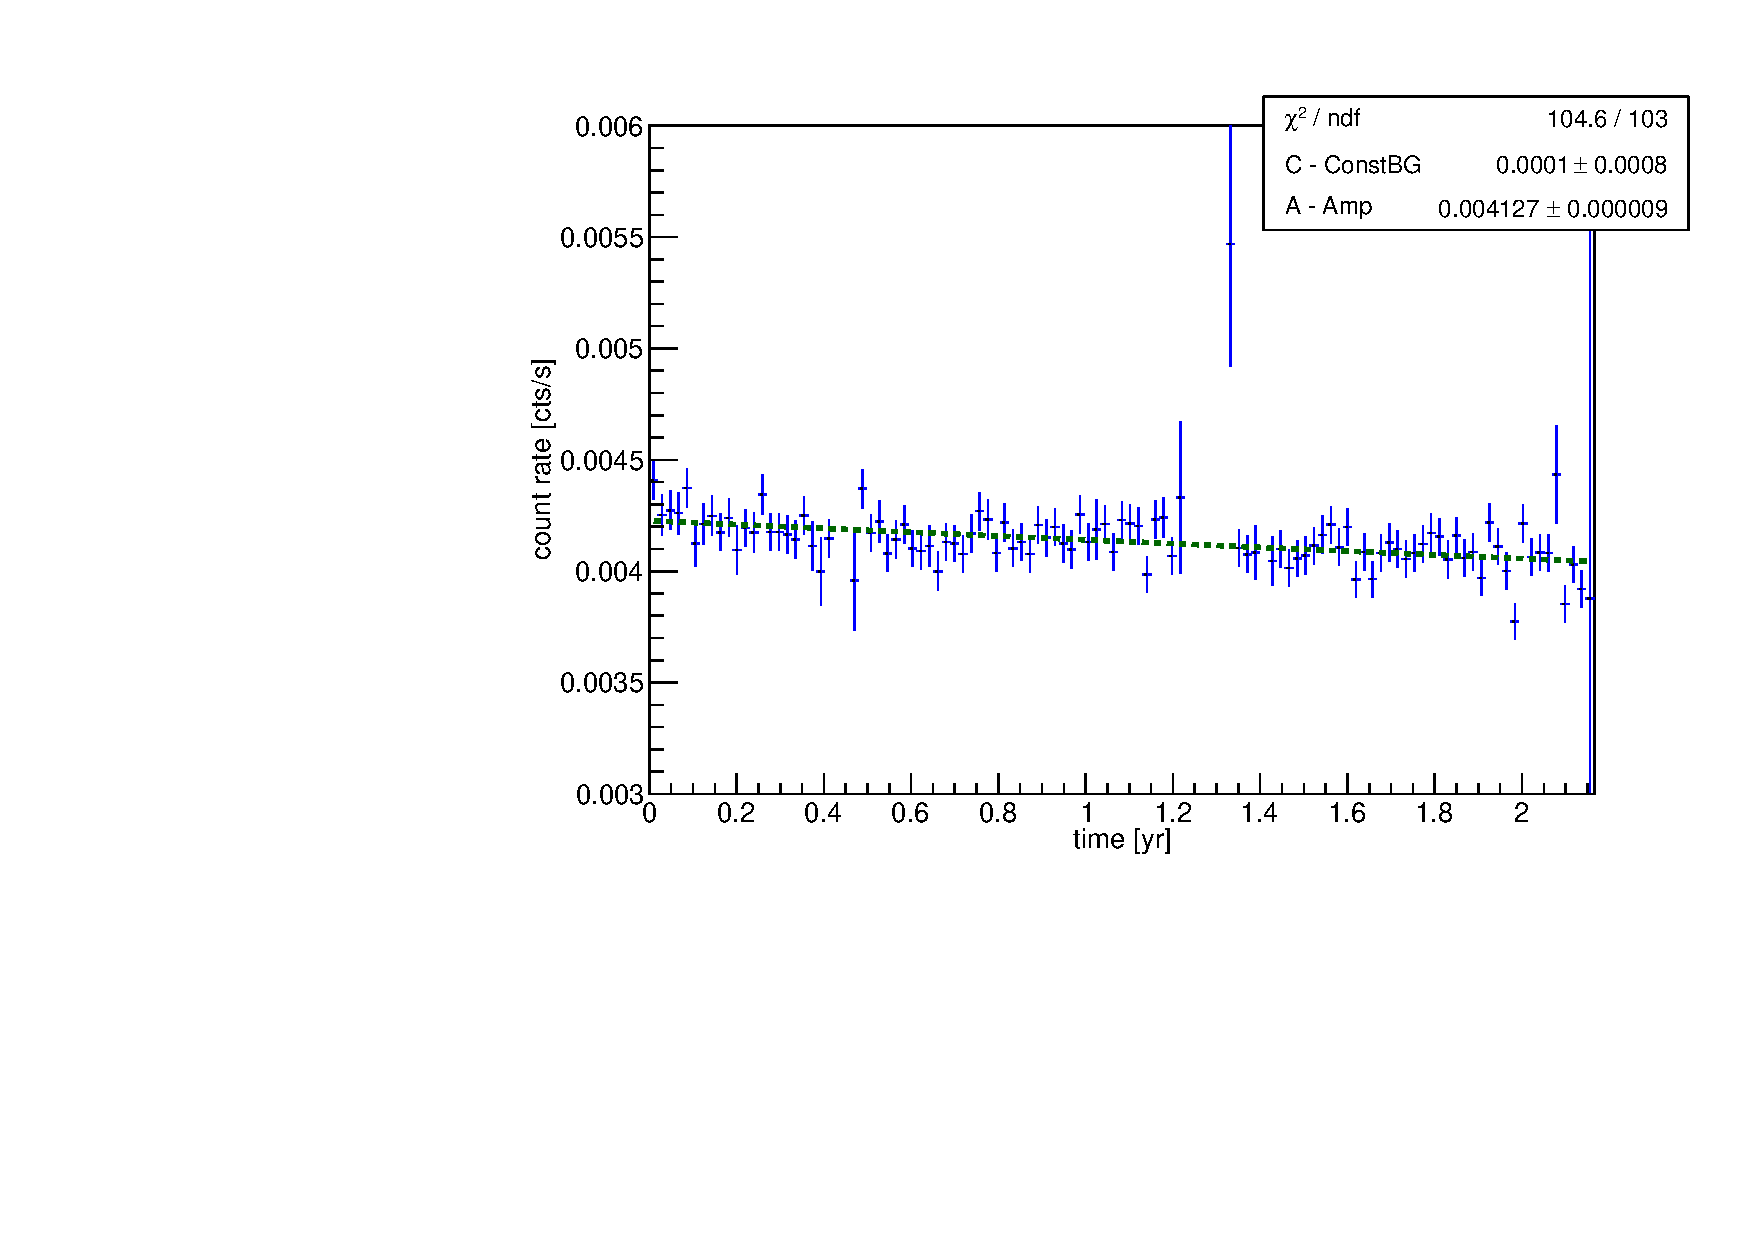
\includegraphics[width=\textwidth]{./Bilder/Argon.pdf}
		\caption{
			Count rate of measured events between 200 and 400 keV over the course of \PII.
			A continuous change in rate can be seen. 
			One can now apply a fit using function \ref{equ:FitFilters2} and through it determine the count rate of \Kr\ at the start of \PII.
		}
		\label{fig:Argon}
	\end{minipage}
\end{figure}























\section{Monte Carlo simulation}
\label{sec:MonteCarlo2}

The second and last value needed to determine the specific activity of \Kr\ is the conversion factor $1/\epsilon V_{\mathrm{sim}}$.
To obtain this conversion factor, almost the same process has to be applied as for line count rate analysis, with the only difference that this time the \Kr\ decays themselves are simulated instead of 514 keV gamma.
\\

A problem is, however, that detector efficiency of \Kr\ can be expected to be very small.
This is due to the beta electrons of the \Kr\ decay having a low probability of actually being detected.

On the one hand, electrons emitted far away from the detectors have a longer distance to travel in which they lose a lot of energy by generating scintillation light.
This effectively reduces their range and therefore their probability of even been detected.

On the other hand, electrons only have a small transmission factor in germanium.
This causes a significant number to be absorbed in the dead zone of the detectors where they do not generate any measurable signal.
In comparison, the 514 keV gammas have a large transmission factor that allows them to deposit their energy deep in the active volume of the detectors.
\\



That is why a far bigger number of N = 1 billion \Kr\ decays in a volume of again $V_{sim} = 17.65 \mathrm{m}^3$ were simulated.
From the simulated events  a combined spectrum of the measured \Kr\ beta electrons plus the 514 keV gammas can be created which can be seen in figure \ref{fig:Sim1Spektrum}.
\\

One can now compare this spectrum with figure \ref{fig:PhasenraumMC514} of the first Monte Carlo simulation.
It is of interest to find out how large the share of events generated by the beta electrons of all measured events is in the range of interest.
If their contribution to the spectrum were too big some corrections have to be made on the resulting detector efficiency as the simulation only estimated the volume of the dead layer creating an error.
To evaluate the betas contribution a comparison value has to be found.
Such a value can be generated by using the 514 keV gamma peak.
This peak can be used as a normalization factor.
When tanking the sum of all events measured in the range from 200 to 400 keV and dividing it through the number of line counts of the 514 keV peak one results in value $N_{\mathrm{sum}}/N_{\mathrm{peak}} = 2.481$ for the first and $3.137$  for the second simulation.
The value of the first simulation represents the relative amount of gamma events in 200 to 400 keV range per 514 keV line count whereas the value from the second simulation represents the ratio of all \Kr\ caused events per line count.
This means that one can determine the relative contribution of the gamma events in the second simulation by dividing the first value through the second value.
This results that a majority of $79.1 \%$ of all events measured in the 200 to 400 keV range were actually caused by gammas whereas only a smaller amount of $20.9 \%$ were caused by the released beta electron.
Due to the fact that the correction on the detector efficiency would have only change
\\

When compare this spectrum with the one determined for the other Monte Carlo simulation you can see these two spectra look relatively similar.
To test this one can calculate a ratio from the two spectra and compare them.
An appropriate ratio for the range of values of this analysis would be to take the sum of all events with an energy between 200 and 400 keV $N_{\mathrm{sum}}$ and divide by the counts in the 514 keV peak $N_ {\mathrm{peak}}$.
This results in a value of $N_{\mathrm{sum}}/N_{\mathrm{peak}} = 2.481$ for the first simulation and $3.137$ for the second simulation.
Due to the fact that the first simulation only computed 514 keV photons the first value represents the ratio when only the 514 keV photons would contribute to the energy spectrum.
The second value, on the other hand, represents the ratio when the 514 keV photons together with the electrons generate the spectrum.
This means that the electrons only generate about 20$\%$ of all measured events in the range of 200 to 400 keV.
The 514 keV photons created the rest.
\\

This is actually an advantage.
If the majority of the measured events were created by electrons then one would have to apply a correction onto the detector efficiency.
This is because of a weakness of the simulated detectors.
The dead layer of the actual detectors isn't known that well which is why the simulated detectors can only work with an assumptions of the actual dead volume of the detectors.
Unfortunately, it's hard to correct the determined value for this weakness.
It is therefore lucky that the 514keV photons are responsible for the majority of counts in the spectrum and no such correction has to be applied.
\\

But this conclusion of photons being the main cause of the spectrum assumes that in both simulations the same environmental conditions and \Kr\ characteristics were simulated.
Whether this is true or not can easily be determined by looking at line count of the characteristic 514keV peak.
In the case of the first simulation an amount of 10179 events were measured by the BEGe detectors in the 514keV peak with a decay density of about 2832 $\unit{photon}/\unit{l}$.
On the other hand in the second simulation only 817 events were measured with a decay density of 56640$\unit{decay}/\unit{l}$.
But one has to consider that in the case of the first simulation only the photons of the \nuc{Rb}{85m} relaxation were emitted and \Kr\ only decays into this exited state with a probability of 0.434$\%$.
The effective decay density of the first simulation is therefore about 652511 $\unit{decay}/\unit{l}$.
To compare these two line counts, one now has to scale one of the two line counts so that the same decay density can be assumed.
By applying the scale of $\frac{56640}{652511}$ onto the amount of events in the 514keV peak from the first simulation you get a adjusted value of 884 events.
The fact, that this value is roughly the same size as the value 817 form the second simulation, proves, that a similar environmental situation and \Kr\ characteristics must have been simulated.
This conclusion also justifies retroactively the simplification in the first simulation where only photons of the \nuc{Rb}{85m} were emitted to replace the computation of the actual decays.
\\

Now to calculating the conversation factor from this simulation.
This requires determining the number of events with an energy in the range 200 to 400 keV and the untriggered detector anticoincidence veto.
In this case an amount of $\Delta N$ = (1438$\pm$38) events was determined.
With the absolute amount $N_{\mathrm{sim}}$ of decays simulated we determine a detector efficiency of
\begin{equation*}
\epsilon = \frac{\Delta N}{N_{\mathrm{sim}}} = (1.438\pm0.038)\times10^{-6} \frac{\unit{event}}{\unit{decay}}
\end{equation*}
This values says that any decay in the liquid argon has a probability of $\epsilon$ to be measured by one of the detectors that was always on.
With this value one can again calculate the volume independent conversation factor
\begin{equation*}
\frac{1}{\epsilon V_{\mathrm{sim}}} = (39.38\pm1.04) \frac{\unit{decay}}{\unit{event} \times \unit{l} }
\end{equation*}
With this conversation factor one can now finally calculate the specific activity of \Kr.
By applying equation \ref{equ:ActivityDieZweite} and feeding it with the values found we result in an specific activity of $a(t=0) = (61.4\pm41.9) \frac{\unit{mBq}}{\unit{l}}$ at the start of Phase II.

One can now get back to the graph \ref{fig:ChangeInEventRateFit}, subtract the constant background of each point and scale each value by the conversation factor.
The resulting graph can be seen in figure \ref
Now it is of interest to compare this value to the specific activity found in the line count rate analysis.
For this one has to calculate the mean specific activity over all of Phase II.
This can easily be done by integrating an exponential decay function over all of \PII\ and then dividing it by 2.17 yr.

\begin{equation*}
\bar{a} = \frac{1}{2.17\unit{yr}} \int_0^{2.17\unit{yr}} a(t=0)\times\exp \left( \frac{\log(2)}{T_{\frac{1}{2}}} t \right) \mathrm{d}t
\end{equation*}

with $T_{\frac{1}{2}}$ being the half life of \Kr.
This results in an mean specific activity of $ \bar{a} = 57.294 \frac{\unit{mBq}}{\unit{l}}$.
\\

When comparing the here obtained result with the specific activity found in the line count rate analysis you will realize that there is a problem.
The mean specific activity of all investigated detectors found in the first method had a value of $\bar{a} = (0.508\pm0.086)\frac{\unit{mBq}}{\unit{l}}$.
Compared to this is the value determined here is two orders of magnitude bigger.
This is problematic.
The critical question are now: 
Which of the methods is faulty, which of the assumption used was wrong and can one still make a statement about \Kr\ specific activity from the problematic approach.
These question will be answers in the following section.
\\



In the previous chapter using the line count rate has already shown the specific \Kr\ activity in the LAr to be in the order of 10$^{-4} \unit{Bq}/\unit{l}$,
However, when compared to \nuc{Ar}{39} ($T_{\frac{1}{2}} = 269\unit{yr}$) \cite{singh_nuclear_2006} having a relatively constant specific activity in the order of 1$\mathrm{Bq}/\unit{l}$ hardly any change in count rate made from \Kr\ should be able to be measurable due to it having a count rate four orders of magnitude smaller than the constant count rate of \nuc{Ar}{39}.
But if one were to actually measure a remarkable change due made by \Kr\ decays, one could use this result to falsify the value calculated in the first method.
\\

This process, however, assumes that \Kr\ is the only radioactive isotope with a notable change in its count rate meaning that it has the smallest half life to show any change over the time frame of \PII.




To actually measure the change in the count rate, the count rate must be drawn over time and an exponential fit function applied through it.
From the amplitude of the exponential function the value $R_{\mathrm{count}}(t=0)$ of counts per second at the start of \PII\ can be determined.
\\

It is also necessary to use a Monte Carlo simulation to calculate another conversion factor between the measured counts and the number of decays required for them. 
A new Monte Carlo simulation must be used, since in this case all \Kr\ must be considered in the simulation and not only the 514 keV gamma.
With this new conversion factor $\frac{1}{\epsilon V_{\mathrm{sim}}}$ the specific activity of \Kr\ can finally be calculated.

\section{Motivation}
\label{sec:motivation}
The resulting specific activity of the approach described above is in actuality the combined specific activity of the whole \gerda\ \PII\ setup and not specifically just \Kr.
The reason why one can expect to determine the individual specific activity of \Kr\ with this approach is that \Kr\ has one of the smallest half-lives ($T_{\frac{1}{2}}$ = 10.739\unit{yr}) of all remaining radioactive isotopes in the LAr. 
In comparison, other radioactive isotopes that are of interest are \nuc{Po}{210} (138 d)\cite{kondev_nuclear_2008} and \nuc{Ar}{42} (32.9 yr) \cite{chen_nuclear_2016} .
\\

Even though \nuc{Po}{210} has a half-life much shorter than \Kr's, most of the events created by it will have an energy much higher than \Kr's Q-value.
It can therefore be assumed that it will only have a negligible contribution to the change in count rate if only event with an energy lower than 400 keV will be considered.
\Kr's Q-value actually lies at 687 keV but it can be expected that the majority of \Kr\ events will have an energy lower then this.
By setting the limit even lower than \Kr\ Q-value of 687 keV, it will also suppresses some of the constant background of events with a higher energy while leaving out only a few \Kr\ decays with higer energies.
\\

\nuc{Ar}{42} has a half life that is in the same order of magnitude as \Kr\ and most of its emitted electrons also have an energy in the same range as \Kr\.
Even though its specific activity has already been determined to be smaller than \Kr's at about $0.148\mathrm{mBq/l}$ \cite{becerici_schmidt_results_2014}, this isotope can still be problematic as it decays into the unstable isotope \nuc{K}{42}.





The motivation behind this approach lies in \Kr\ having a low half life of $T_{\frac{1}{2}} = 10.739\unit{yr}$.
As it will be shown in section \ref{sec:motivation} it is one of a few isotopes that should show a notable change over the time scale of \PII.









Right after its creation \nuc{K}{42} is positively ionized as the electron also created in the beta decay escapes due to its high energy.
These positively ionized \nuc{K}{42} atoms will then be attracted by the electrostatic fields of the germanium detectors.
This results in a higher \nuc{K}{42} density around the detectors.
%This, however, makes it impossible to calculate a detector efficiency for \nuc{K}{42}  as it is no longer homogeneously distributed in the LAr tank. 
\nuc{K}{42} also has a half life of 12.355 h \cite{chen_nuclear_2016}.
It is therefore to be expected that \nuc{K}{42} has the same activity in the LAr tank as \nuc{Ar}{42} because compared to to \nuc{Ar}{42} it decays instantaneously.
However, due to its higher density around the detectors a much higher specific activity can also be expected to be measured in the detectors.
Because of this one can assume that it will also show a much bigger change in the count rate than expected.
This could mean that it might even dominate over \Kr\ change in count rate.
How much of an impact it will actually make on the change in count rate is hard to approximate.
However, if a notable change in count rate was able to be measured it might not even have to be caused by the \Kr.
In this case the change in count rate will be fitted with two different fit functions - on with a fixed half life of \Kr\ and one with a fixed half life of \nuc{Ar}{42}.
Depending on which of the fits is better suited for the measured data it will be decided whether \Kr\ or \nuc{Ar}{42} is responsible. 

\\



\section{Count Rate}
\label{sec:EventAct}

\begin{figure}[t!]
	\centering
	\begin{subfigure}{.475\textwidth}
		\centering
		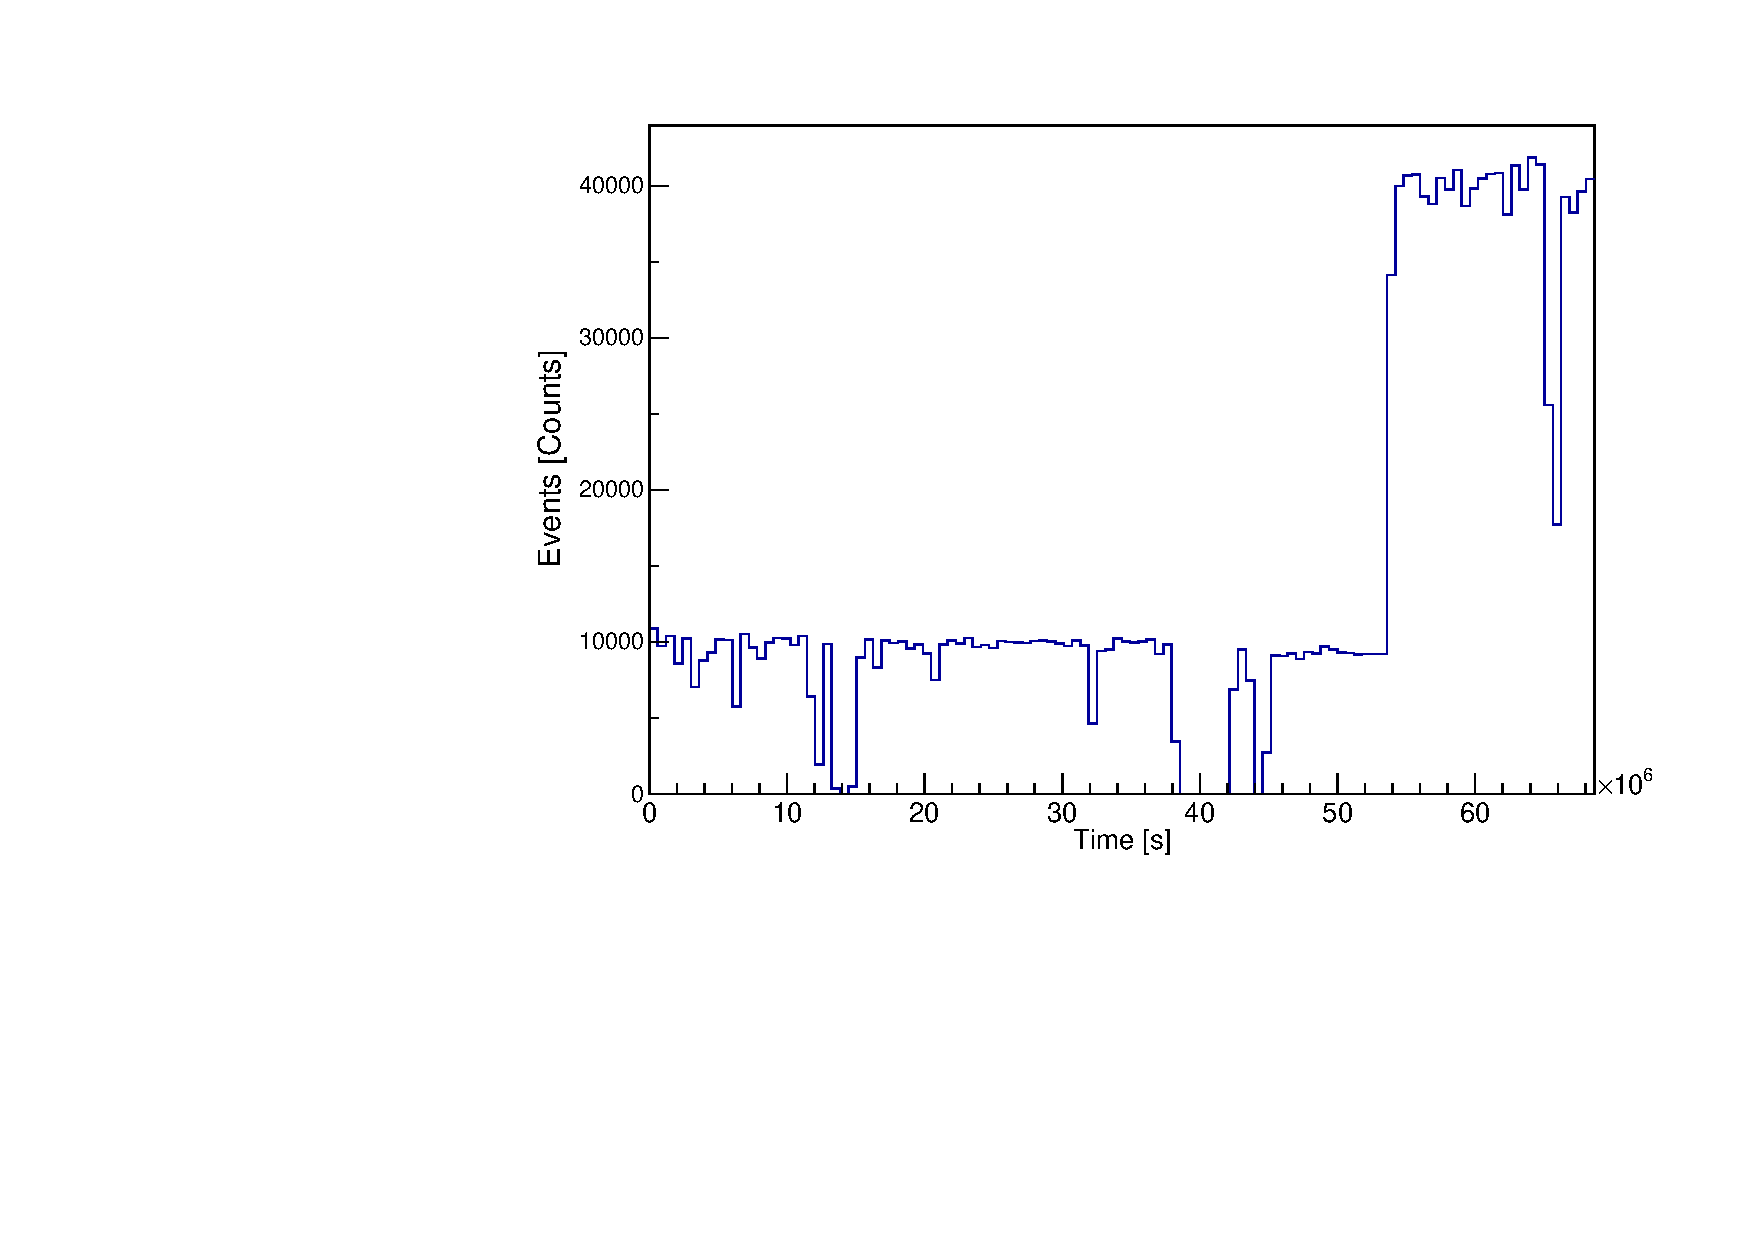
\includegraphics[width=\textwidth]{./Bilder/ZeitverlaufALLE.pdf}
		\caption{energies lower than 400 keV}
		\label{fig:ZeitAll}
	\end{subfigure}\hfill%
	\begin{subfigure}{.475\textwidth}
		\centering
		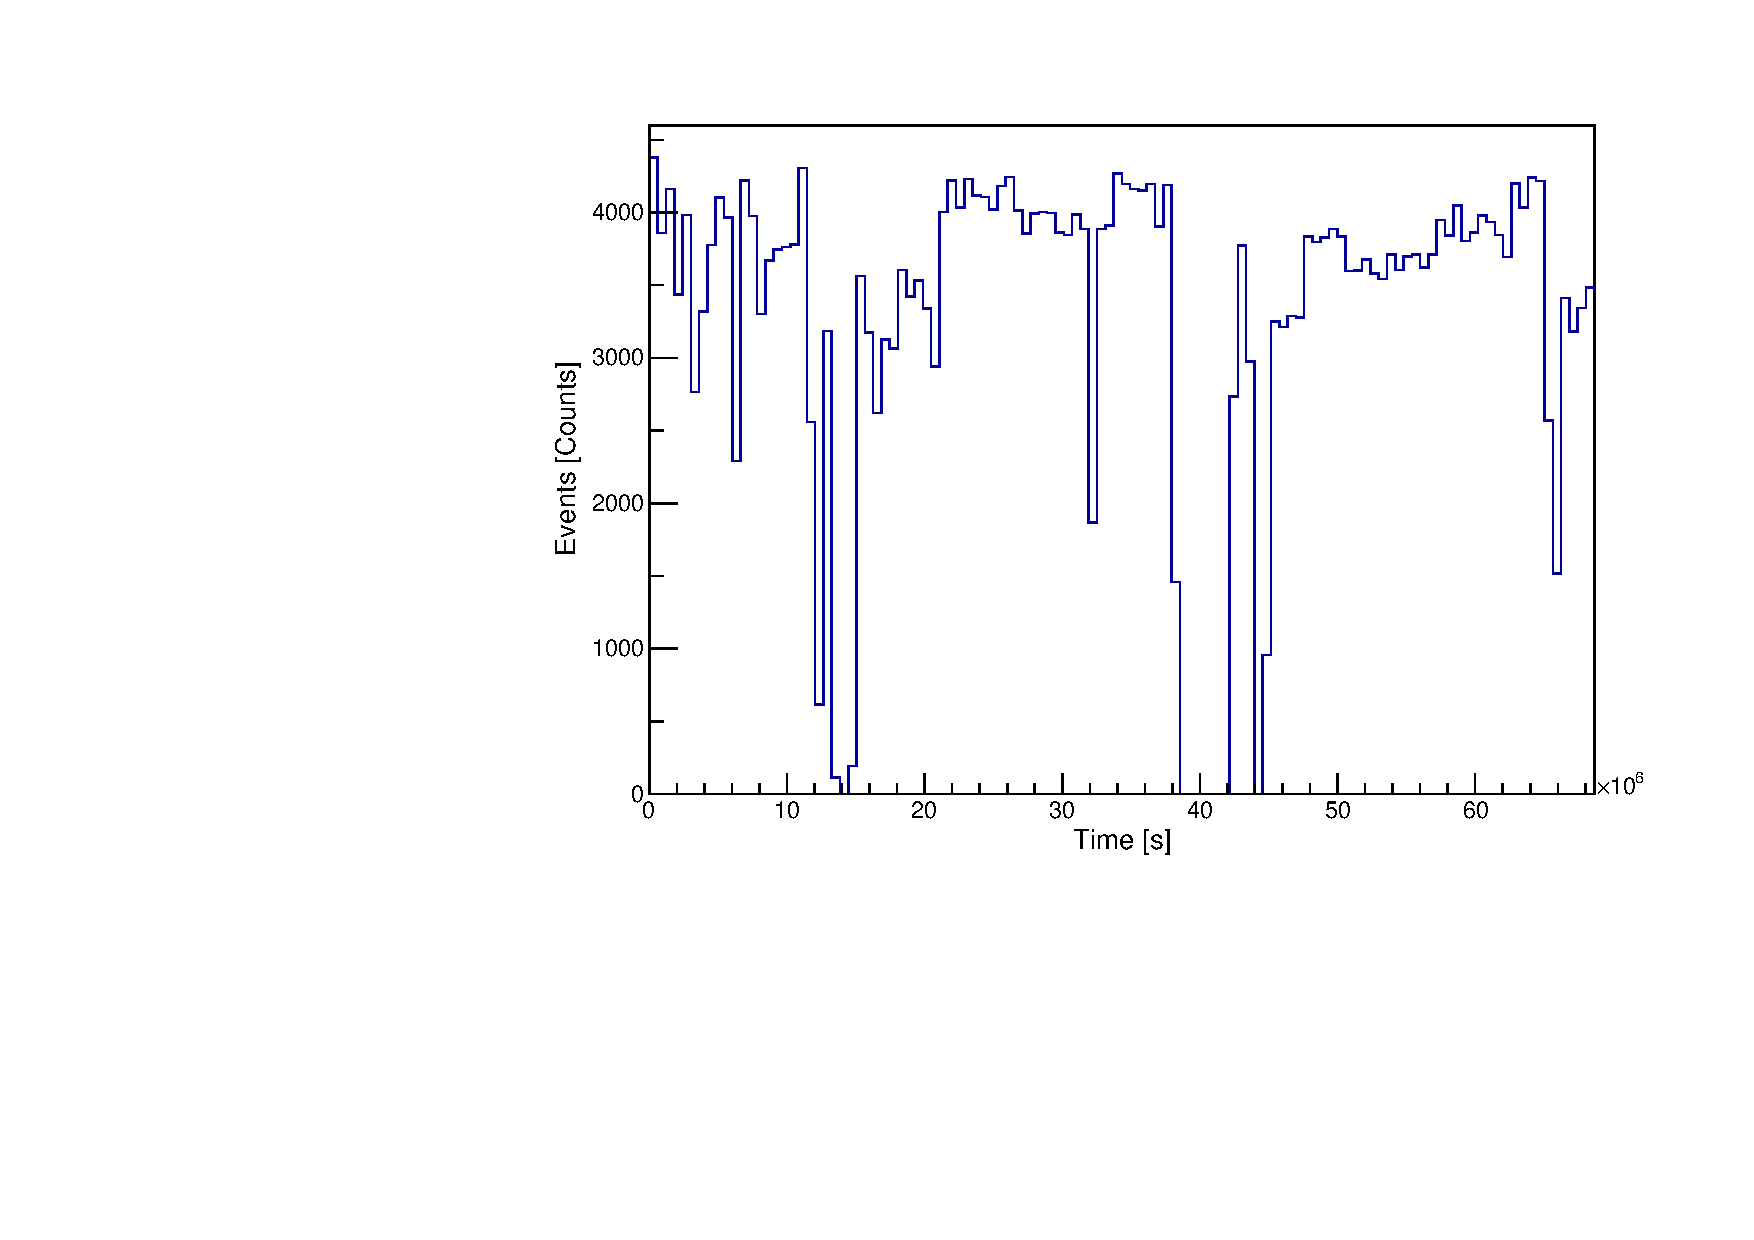
\includegraphics[width=\textwidth]{./Bilder/ZeitverlaufLimits.pdf}
		\caption{energies between 200 and 400 keV}
		\label{fig:ZeitLimits}
	\end{subfigure}
	\\
	\caption{
		The change of count rate over time.
		In both figures the amount of counts measured in one week are plotted over the whole time frame of \PII. 
		The binning of these hisograms was chosen to be one week per bin which results in about 113 bins over all of  \PII.
		In figure (a) no filters were imposed onto the used events while in (b) only those events were used that have an energy between 200 and 400 keV. 
		One can see that further precautions must be taken before an exponential decrease can be determined. 
	}
\end{figure}

To determine the change of count rate over time it is necessary to plot the amount of measured counts over time in a histogram (see figure \ref{fig:ZeitAll}) and later divide those counts by the mean measuring times inside the respective bins of the histogram.
The data used in this approach is the \gerda\ \PII\ data from run 55 to 92.
The used data had also been cut again by the standard \gerda\ analysis cuts (quality, muon, anti-coincedence).
The anti-coincidence cut here also because not only the gammas basically always deposit all their energy in one detector but due to the low  $Q_\beta$ of the \Kr\ the released beta as well.
\\

Figure \ref{fig:ZeitAll} shows the amount of counted events with an energy below 400 keV in each individual week.
From it a jump in the count of events in the second half of \PII\ can be seen.
However, this discontinuous change makes it impossible to determine the change in the counting rate, as no fit function can be applied through the resulting counting rate diagram. 
It is therefore necessary to find a way to suppress this jump, but to do so, its origin must be investigated.
\\

This jump occurs on the 12.10.2017.
On this day the lower energy threshold of all detectors was lowered.
This dramatically increased the number of events measured.
Due to every detector having different characteristics, the limit was set for each detector individually.
Before the lowering the highest limit was set at about 140keV for the BEGes and at 185 for the COAX.
After the lowering all event with an energy of at least about 15keV could be recorded by all detectors.
For a graphical representation, see the beginning of the spectra in figure \ref{fig:before} for all events measured before and figure \ref{fig:after} for all events after the lowering of the limit. 
To work around this continuity problem all one has to do is to apply a lower energy limit of 200 keV.
\\


\begin{figure}[t!]
	\centering
	\begin{subfigure}[t]{.475\textwidth}
		\centering
		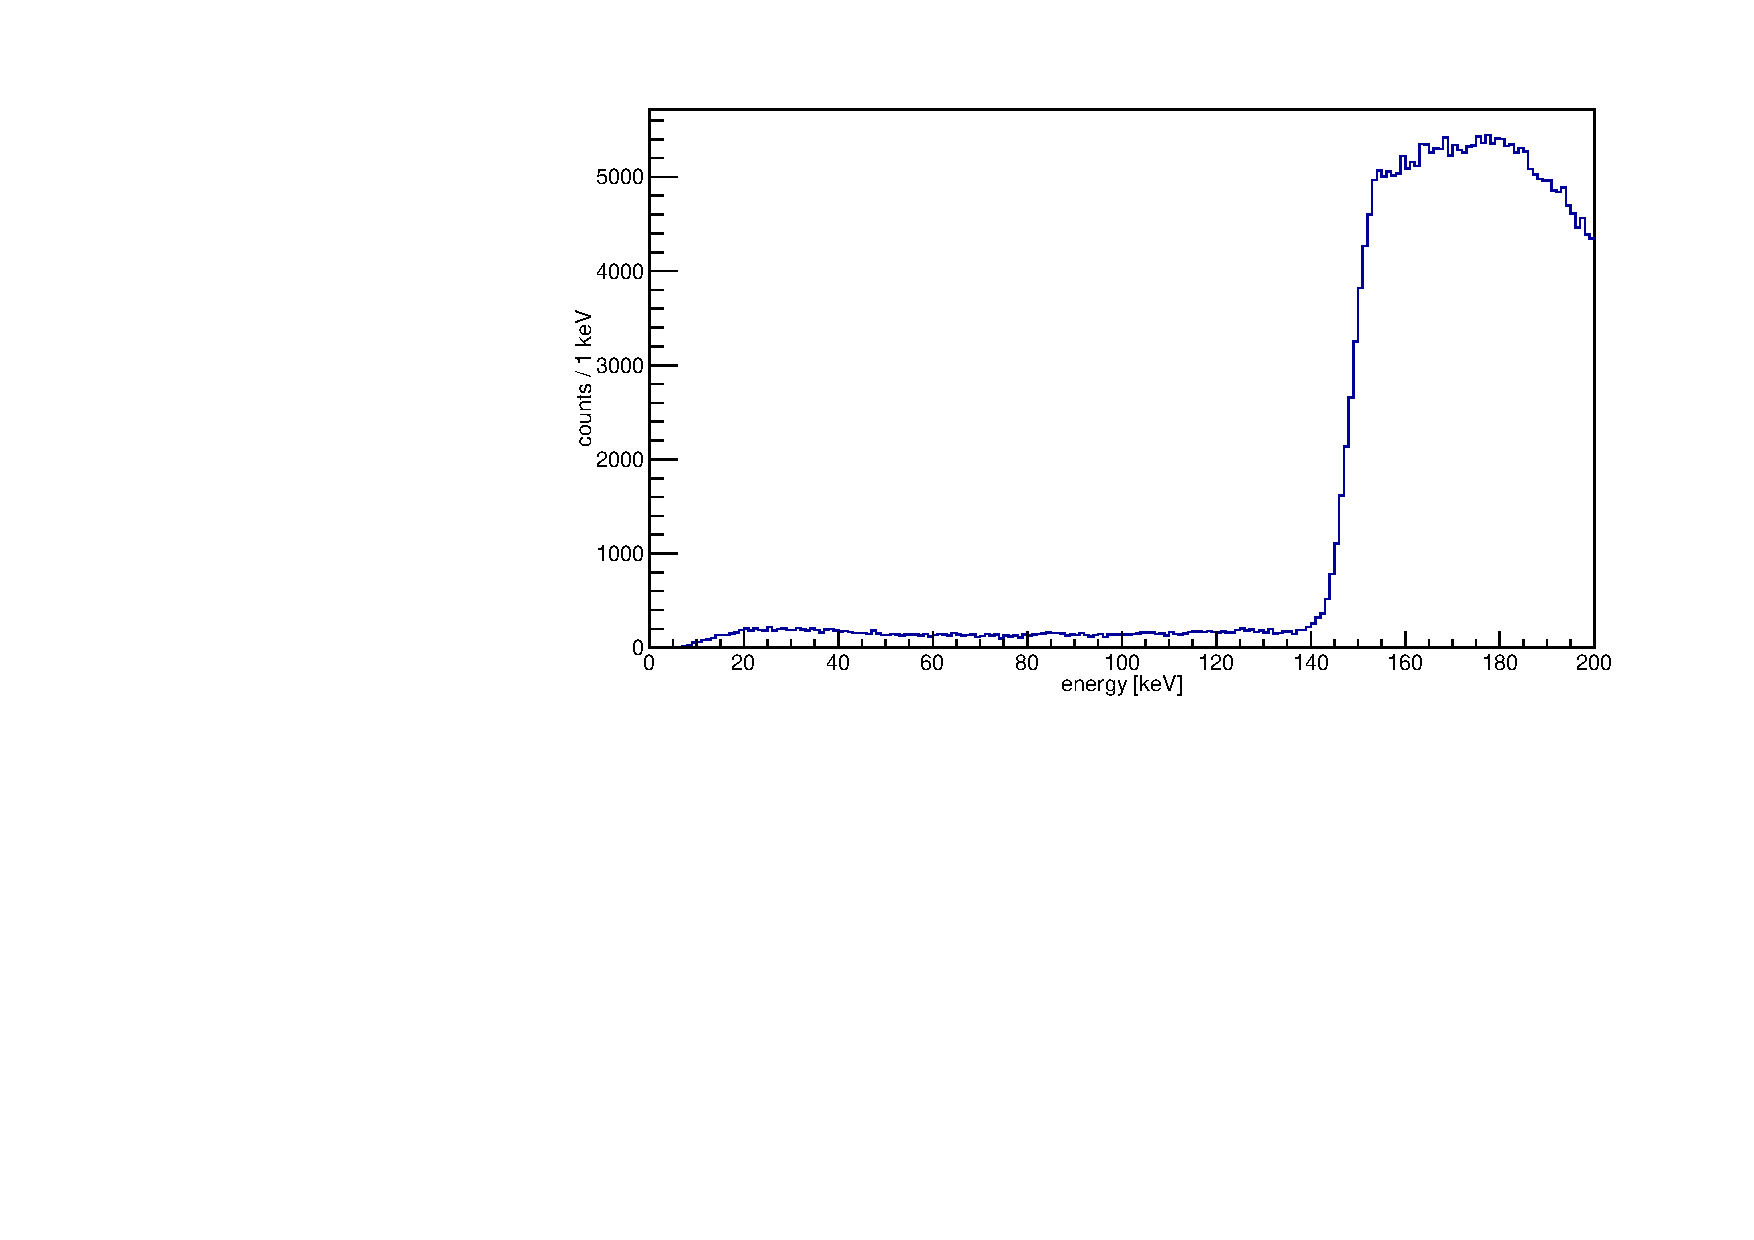
\includegraphics[width=\textwidth]{./Bilder/beforeTheFall.pdf}
		\caption{before}
		\label{fig:before}
	\end{subfigure}\hfill%
	\begin{subfigure}[t]{.475\textwidth}
		\centering
		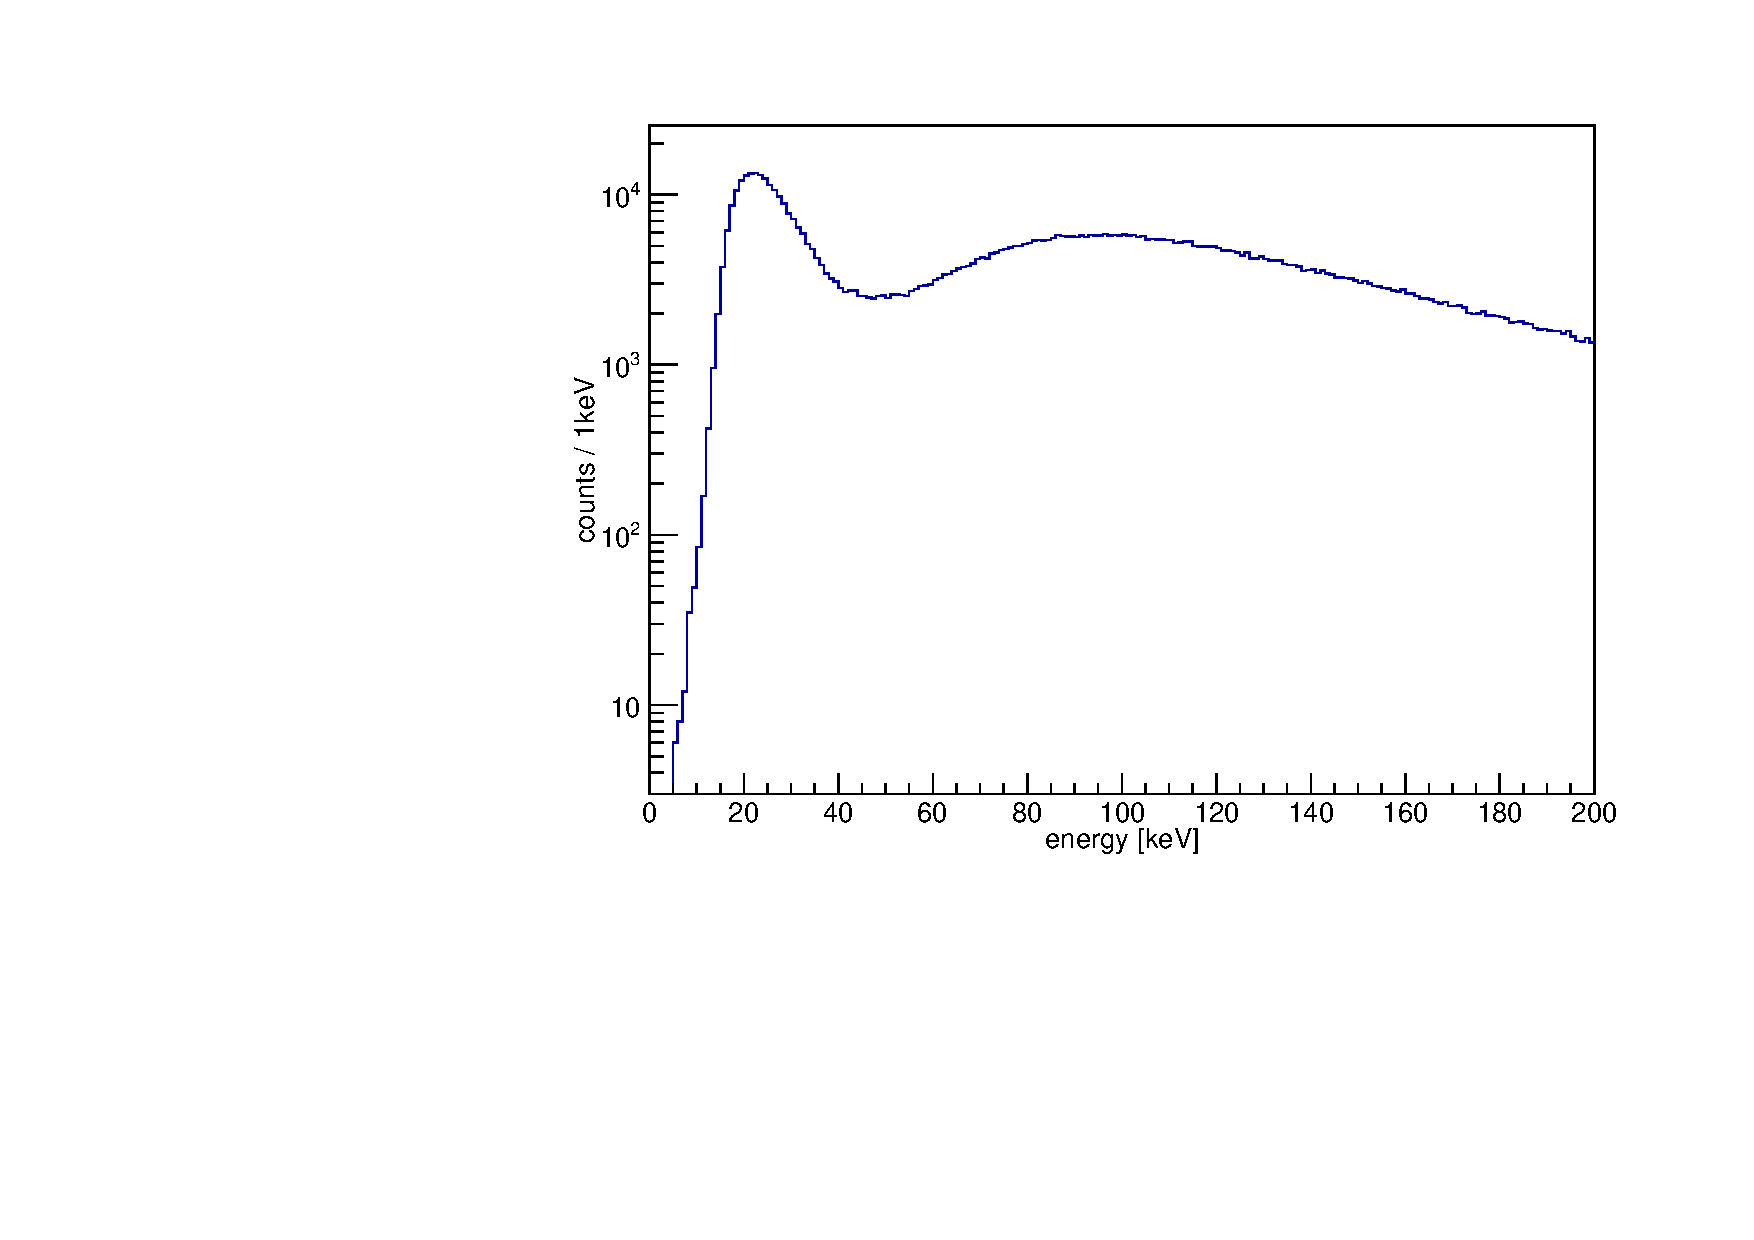
\includegraphics[width=\textwidth]{./Bilder/afterTheFall.pdf}
		\caption{after}
		\label{fig:after}
	\end{subfigure}
	\caption{
		Energy spectra from 0 to 200 keV. 
		Figure (a) shows the resulting spectrum of all events measured before the lowering of the lower energy threshold of recorded events on 12.10.2017 while (b) shows the spectrum after this date.
	}
	\vspace{5mm}
\end{figure}

What must also be taken into account is that the approach through a combined counting rate requires all detectors used for the evaluation to have been continuously measuring throughout all of \PII\.
If at any point one of the detectors stops taking measurements, it would result in a jump in this combined count rate creating discontinuities in its course.    
In the further course of this analysis, therefore, all events are rejected that were measured in a detector whose measurement process was interrupted at some point in \PII.
This retroactively also explains why the data of \gerda\ run 53 and 54 have been disregarded.
In these two runs, a smaller number of detectors were measuring than usual.
This would result in a small pool of detectors with an uninterrupted measurement process available and therefore less data being rejected.
By discarding the data of run 53 and 54 more detectors can be used in the analysis and therefore more data.
The resulting count histogram considering the upper and lower energy limit and only using data from continuously measuring detectors can be seen in figure \ref{fig:ZeitLimits}.
\\

The count rate of each individual week can now be determined by dividing histogram \ref{fig:ZeitLimits} by the mean measuring times of each week in histogram.
To determine these mean measuring times the test pulse signal can be used again.
Similar to how it was done in the line count rate analysis for each week the number of recorded test pulse signals can be determined and their individual amount multiplied by 20 s.
Using this procedure results in a histogram as seen in figure \ref{fig:effectiveMeasuringTimes}.
\\

\begin{figure}[t!]
	\centering
	\begin{minipage}[t]{.475\textwidth}
		\centering
		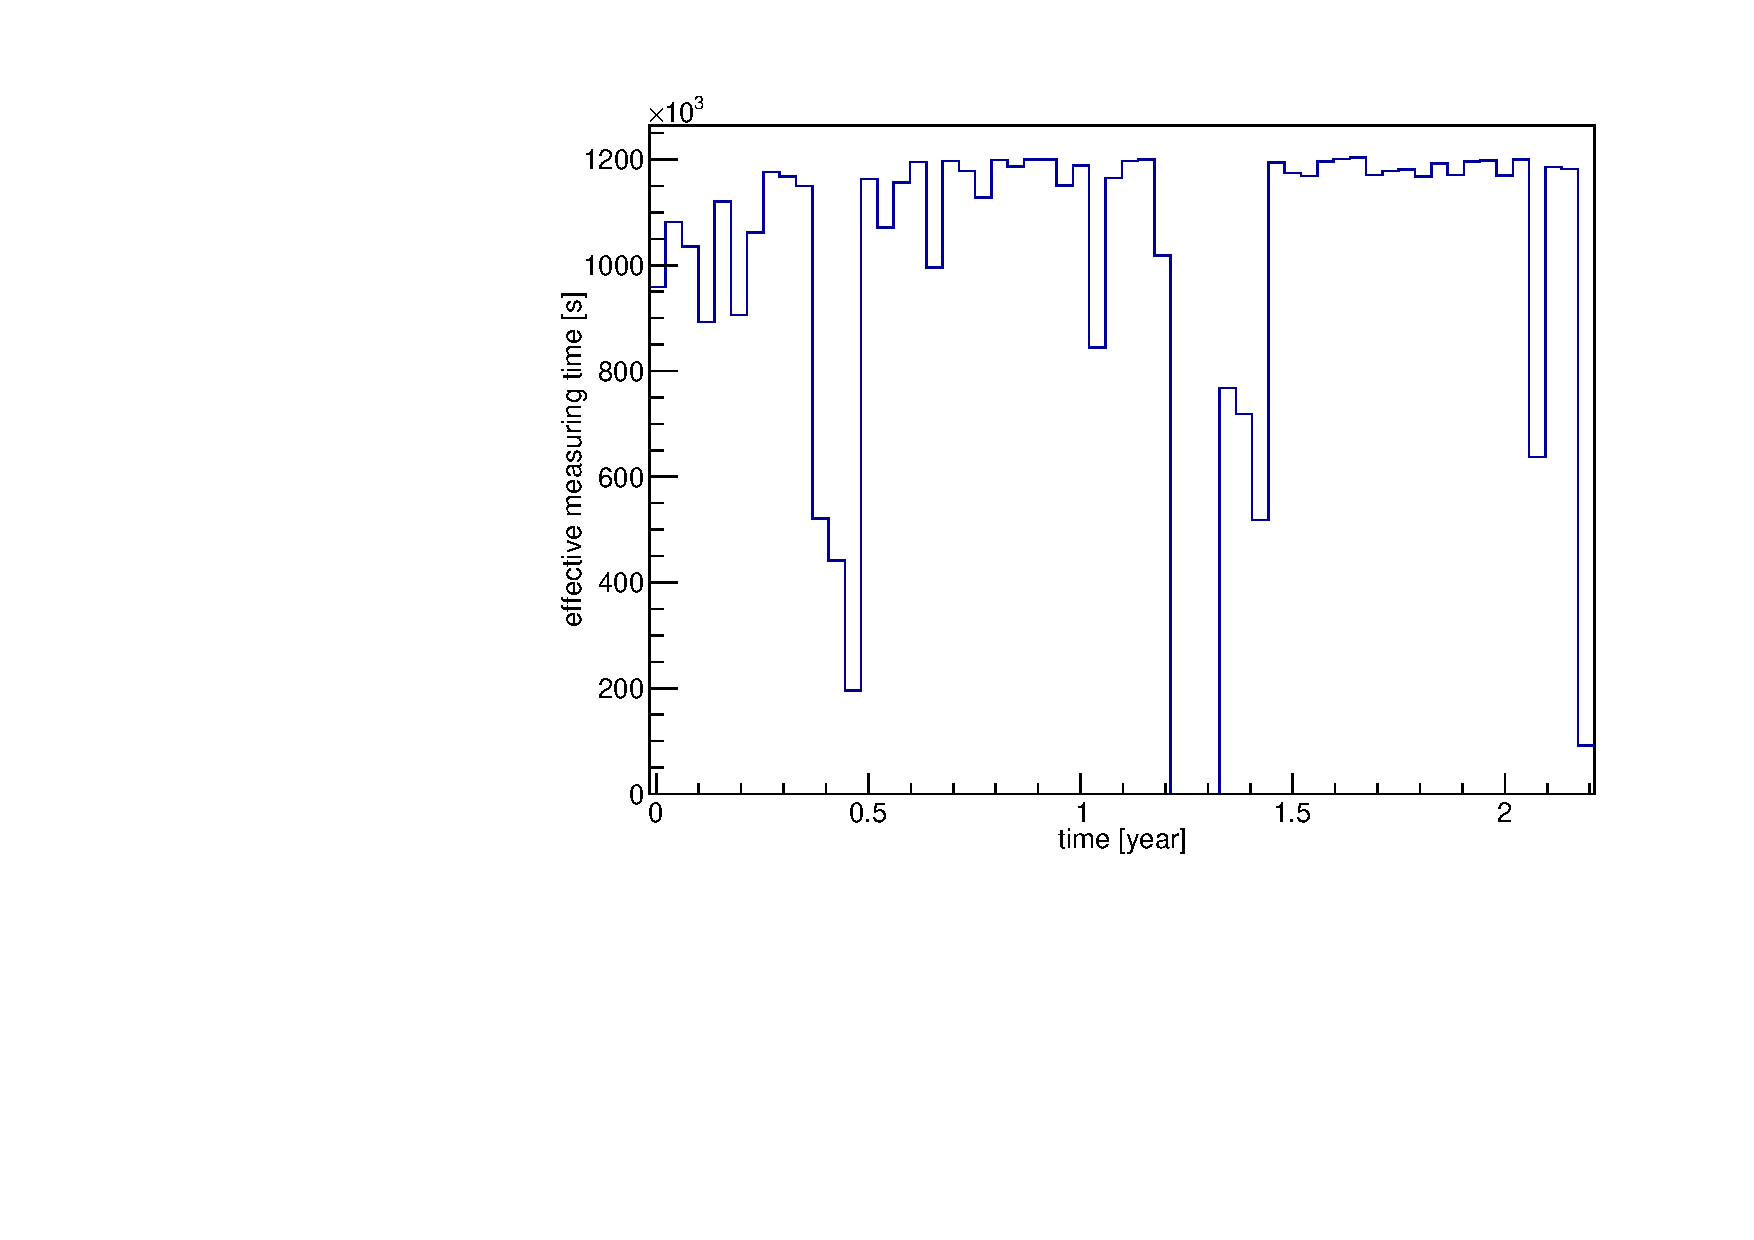
\includegraphics[width=\textwidth]{./Bilder/testpuler.pdf}
		\caption{
			Histogram showing the mean measuring time of each week corresponding to the individual bins.
			Those were determined by the amount of test pulse signals measured in the time frames and their amount multiplied by 20s.
			One can see, that the measuring time of each week varied on a broad level.
		}
		\label{fig:effectiveMeasuringTimes}
	\end{minipage}\hfill%
	\begin{minipage}[t]{.475\textwidth}
		\centering
		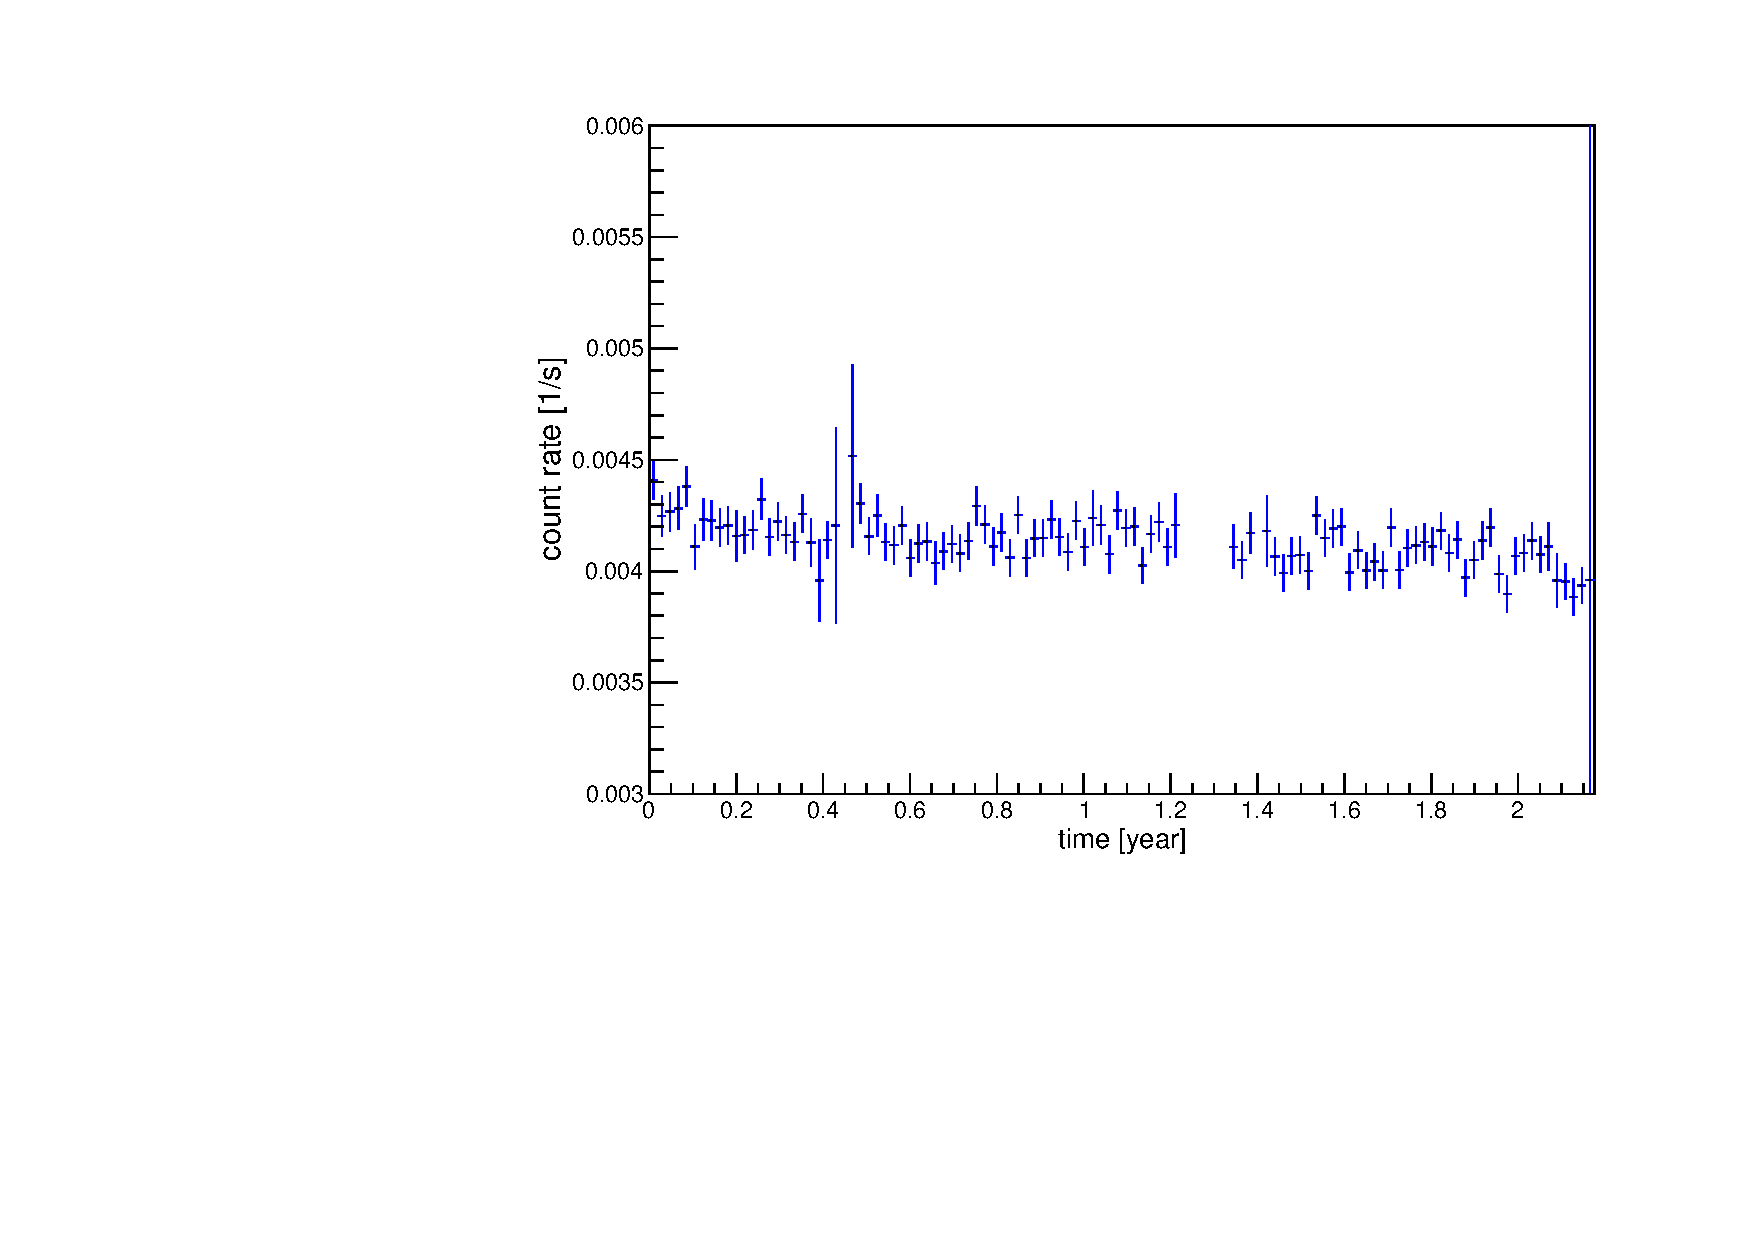
\includegraphics[width=\textwidth]{./Bilder/eventRate.pdf}
		\caption{
			Count rate of measured events between 200 and 400 keV over the course of \PII.
			A continuous change in rate can be seen. 
			One can now apply a fit using function \ref{equ:FitFilters2} and through it determine the count rate of \Kr\ at the start of \PII.
		}
		\label{fig:ChangeInEventRate}
	\end{minipage}
	\\
\end{figure}

Figure \ref{fig:ChangeInEventRate} finally shows the resulting count rate measured over the course of \PII.
This graph can now be fitted with fit function
\begin{equation}

\end{equation}
Fit parameter A corresponds to the initial count rate caused by the decay of \Kr\, B to \Kr's half-life, and C to the constant background rate.
Fit parameter B was fixed to \Kr's half-life of \(10.739\unit{y}\) , but all other parameters remained free, only limited by the condition of them being positive.
The resulting fitting plot can be seen in figure  \ref{fig:ChangeInEventRateFit}.
The only parameter of interest for further analysis is the parameter \(\mathrm{A}\). 
It corresponds to a count rate  
\begin{equation*}
R_{\mathrm{count}}(t = 0) = (1.495\pm0.227) \times 10^{-3} \frac{\mathrm{cts}}{\unit{s}}
\end{equation*}of \Kr\ decay caused events at the start of \PII\.

\begin{table}[t!]
	\centering
	\begin{tabular}{|l|c|}
		\hline
		Name 	& Value  \\ 
		\hline
		A [1/s] &	(1.521 $\pm$ 0.224)$\times10^{-3}$\\	
		\hline
		B [yr] &	10.739\\	
		\hline
		C [1/s] &	(2.714 $\pm$ 0.210)$\times10^{-3}$\\
		\hline
	\end{tabular}
	\caption{
		Fit parameters of fit function \ref{equ:FitNoFilters} applied on the spectra of the respective detectors.
		Parameter A represents the amplitude of the exponential decay function and B the half life of the decaying isotope.
		fit parameter C is there to handle the constant background created by other radioactive isotopes with much higher half lives.
	}
	\label{tab:FitParZeit}
\end{table}

\begin{figure}[t!]
	\centering
	\ifmakefigures%
	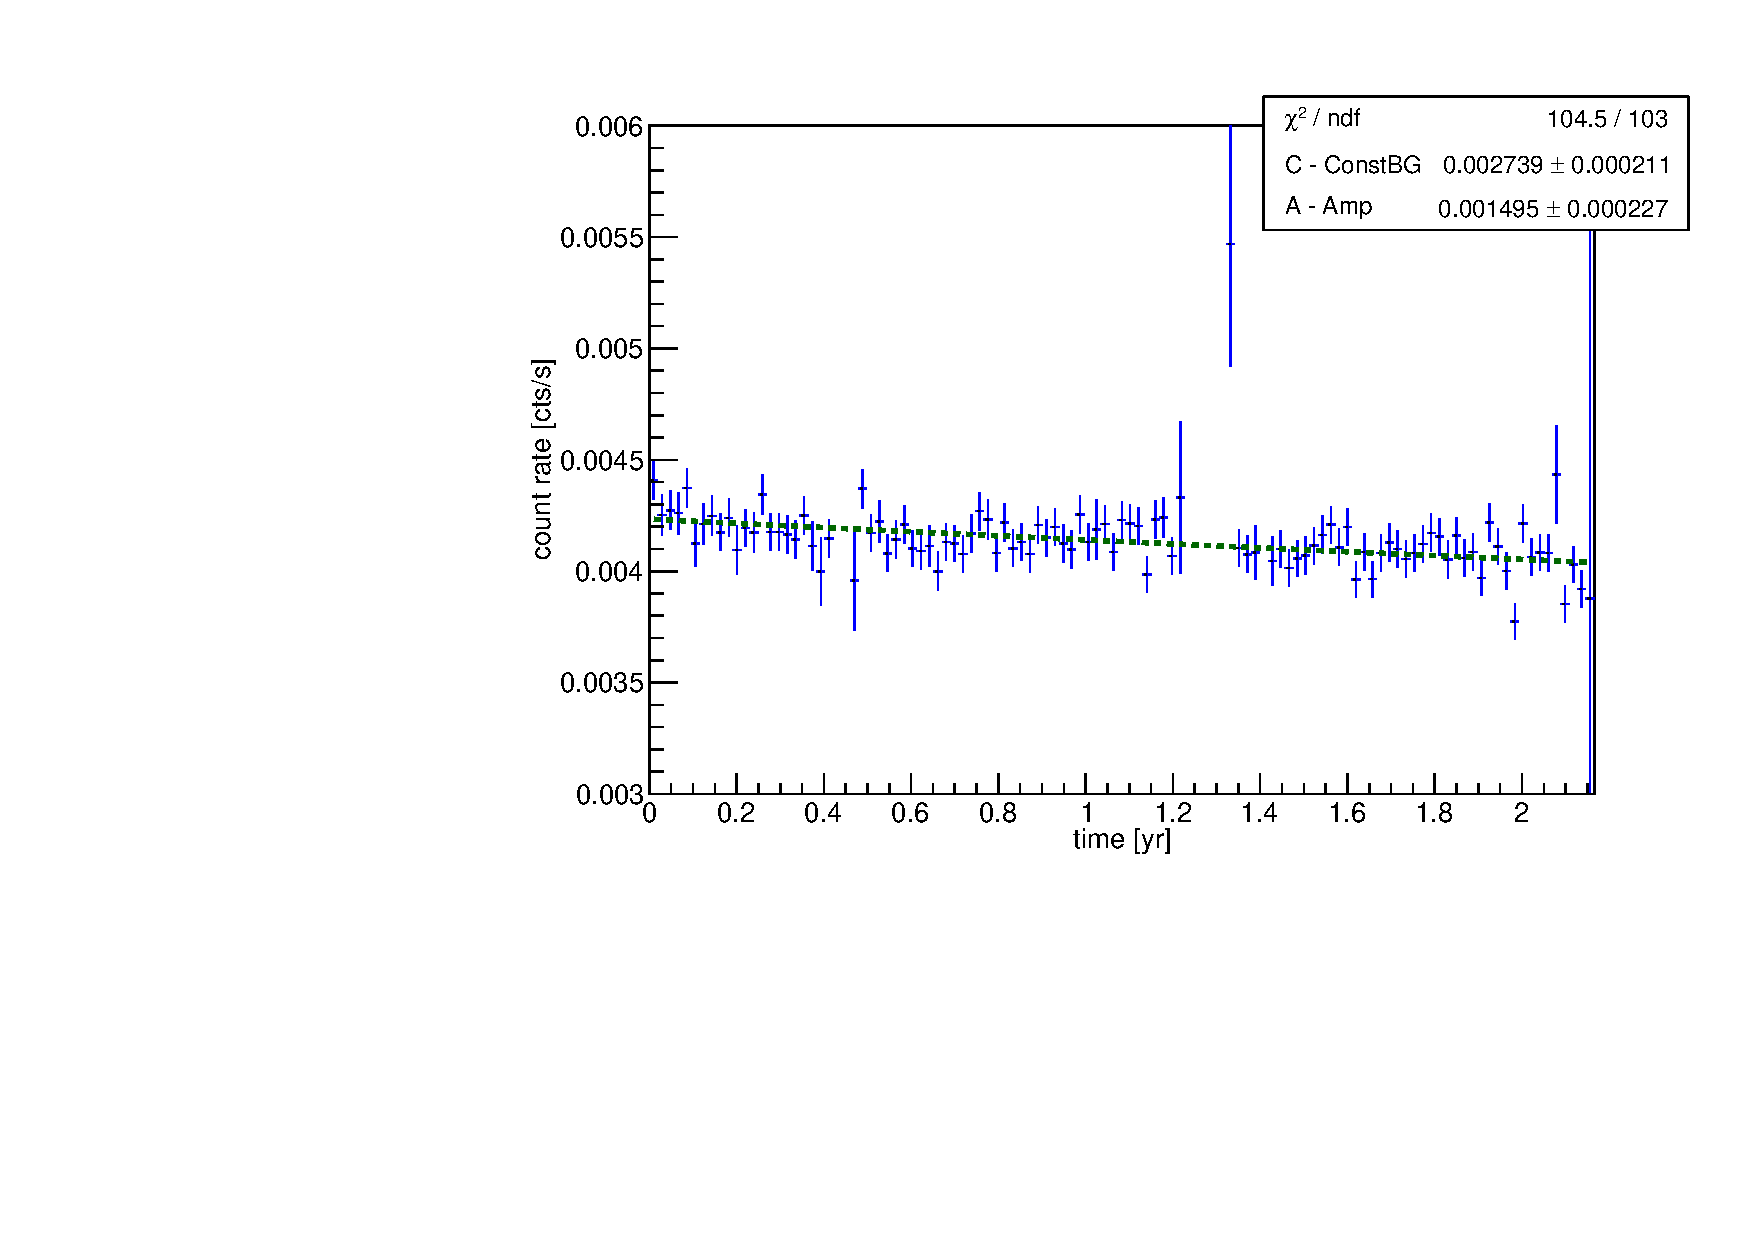
\includegraphics[width=100mm]{./Bilder/eventRateFit.pdf}
	%
	\caption{
		Fitted count rate diagram over the time frame of \PII.
		For the fitting process function \ref{equ:FitFilters2}.
		The resulting fit parameter can be seen in table \ref{tab:FitParZeit}.
	}
	\label{fig:ChangeInEventRateFit}
\end{figure}%

\section{Discussion}
\label{Discussion}

The biggest advantage of the line count rate analysis compared to the second method is that in its case the investigated effect can only originate from \Kr\ and no other isotope.
Because of this the likelihood of its determined value being the actual specific activity is relatively high.
By comparing the results of the first method with those of the WARP and Darkside experiments, you have already seen that the specific activity of \Kr\ is lower than in all other experiments.
The second method however has the problem that theoretically every other isotope that is residual in the LAr contributes to the investigated change over time.
It can therefore be very likely that the mistakes made lies in the assumption that all contribution of any other isotope to this change can be ignored. 
In the beginning of this chapter all isotopes that are the most probable sources of error have already been discussed.
It was already concluded that any contributions from \nuc{Ar}{39} and \nuc{Po}{210} can be disregarded due to their either high half life or their high mean kinetic energy of the escaping particle.
But as it was already indicated there, it might be necessary to discuss the influence of \nuc{Ar}{42} further.
\nuc{Ar}{42} has a half life of 32.9 y which is in the same order of magnitude as the half life of \Kr.
thereforee, one can expect to see a change in its activity over the course of \PII~ of about 4.4$\%$ of its absolute specific activity.
With an specific activity big enough one could expect this isotope to be responsible for the measured decrease.
But due to \nuc{Ar}{42}'s specific activity being much lower than the measured amplitude of $57.294 \frac{\unit{mBq}}{\unit{l}}$  it cannot be the only cause of this .
\\

What is really interesting about \nuc{Ar}{42}, is not the decay of \nuc{Ar}{42} itself, but rather its daughter nuclei \nuc{K}{42}.
\nuc{K}{42} has a half life of 12.355 h \cite{chen_nuclear_2016}.
It can now be approximated, that \nuc{K}{42}'s specific activity is equal to \nuc{Ar}{42}'s specific activity.
This comes from the fact that in comparison to the half life of \nuc{Ar}{42} the resulting \nuc{K}{42} practically decays instantaneously.
This means that it is possible to directly assign one \nuc{K}{42} decay to each \nuc{Ar}{42} that decays.
This doubles the number of decays which can be attributed to \nuc{Ar}{42}.
But assuming that the individual \nuc{Ar}{42} and \nuc{K}{42} isotopes are homogeneously distributed in the LAr, their combined specific activity is still by far not big enough to explain the bigger amplitude measured.
\\

But here lies the critical point.
The \nuc{K}{42} isotopes are in fact not homogeneously distributed in the LAr.
To understand why they are not one has to look at what a \nuc{K}{42} does right after it is formed.
Right after a \nuc{Ar}{42} decays its resulting \nuc{K}{42} isotope positively ionized.
This results from the fact that the newly formed electron escapes from the decay position due to its high velocity.
Now that the \nuc{K}{42} isotopes are positively charged, they can be deflected by an electric field.
\\

Such fields in the LAr tank originated from the germanium detectors.
In a germanium detector it is necessary to create a great electrostatic potential difference between the doped electrodes.
The resulting electric field separates electron-hole pairs that might have been created by other particles depositing their energy in the semiconductor \cite{spieler_semiconductor_2005}.
The field then guids the particles to the respective electrodes and by that creating a current which can be measured externally.
For a high detection efficiency strong fields are necessary.
Otherwise the electron or the hole might recombine in the p-type volume without creating any signal.
\\

The positively ionized isotopes are now deflected by these electrostatic fields to the negatively charged surface of the detectors. 
In the LAr the mean time it takes the ionized \nuc{K}{42} to capture an electron as compensate for its positive charge is relatively long. 
Thats why even though the fields are not very strong far away of the detectors the \nuc{K}{42} can still travel a relatively long distance before it either captures an electron or decays itself. 
Now that the density of \nuc{K}{42} isotopes is higher near the germanium detectors it can be expected that the specific activity around the detector also increases.
\\

The effect explained here has already been measured in \gerda\ and it is actually one of the greatest background sources of the whole experiment.
\nuc{K}{42} has also the unfortunate characteristic for the \gerda\ experiment that its Q-value of about $Q_\beta =3525\unit{MeV}$ lies higher than the Q-value of the double beta decay of \nuc{Ge}{76} $Q_{\beta \beta} = 2039\unit{MeV}$.
This means that electrons of the \nuc{K}{42} decay can create background events in the investigated rage. 
Initially it was not expected to create much background.
Its influence on the measurement however was only recognized after the start of \PI, when its counting rate was higher by a factor of 20. \cite{becerici_schmidt_results_2014}.
Techniques to suppress the background of \nuc{K}{42} were introduced over time like the usage of nylon mini-shrouds (NMS) as a mechanically barrier.
The NMS together with the active filters of the pulse shape analysis and the LAr veto have proven to bee able to suppress \nuc{K}{42} events by more then three orders of magnitude.
\\

In this case however it is not possible for the analysis to use the active filters to suppress the \nuc{K}{42} further.
Otherwise one would also filter out the \Kr\ events that are supposed to be investigated here in the first place.
So it still can be expected that a not negligible proportion of the measured specific activity comes from the denser \nuc{K}{42} in the region of the detectors.
What effective specific activity can be expected from the \nuc{Ar}{42} is difficult to estimate, but you can assume that it should be far greater than that of \Kr.
To get a quantitative approximation, you can use the plot of the event rate change again (see \ref{fig:ChangeInEventRate}) and modify the fit function used so that two exponential decays plus a constant background are taken into account.
Both exponential decay fit functions have their half life fixed to the respective values of \Kr\ (10.739y) and \nuc{Ar}{42} (32.9y).
The used fit function can be seen in equation \ref{fig:doubleFitFun}, the resulting fit function in figure \ref{fig:double} and the fit parameter in table \ref{tab:doubleFitpara}.
\begin{equation}
\mathrm{f}(x) = \mathrm{A}\times\exp\left(-\frac{\log(2)}{\mathrm{B}} x \right) + \mathrm{C}\times\exp\left(-\frac{\log(2)}{\mathrm{D}} x \right) + \mathrm{E}
\label{equ:doubleFitFun}
\end{equation}

\begin{table}[t!]
	\centering
	\begin{minipage}[t!]{.475\textwidth}
		\centering
		\ifmakefigures%
		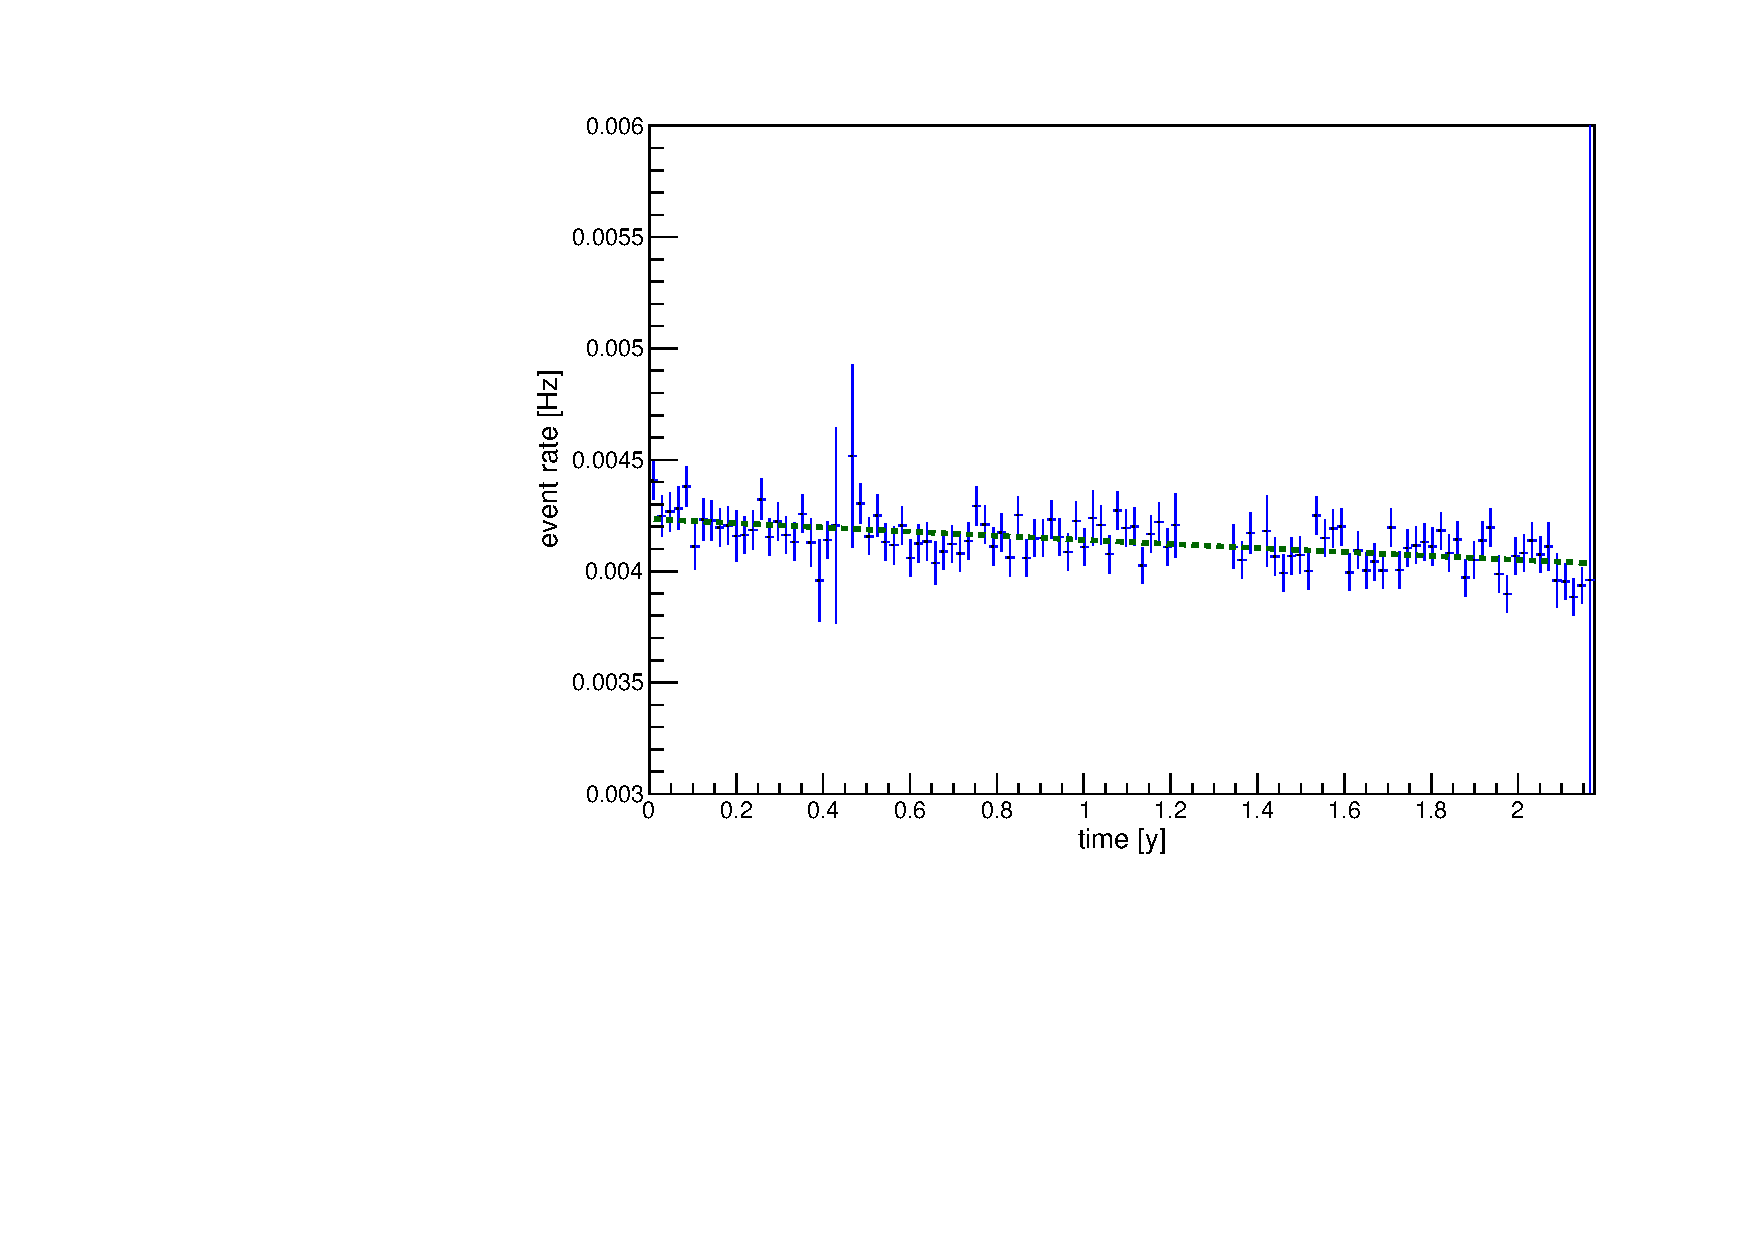
\includegraphics[width=75mm]{./Bilder/doppelt.pdf}
		%
		\captionof{figure}{
			Fitted count rate diagram over the time frame of \PII.
			For the fitting process function \ref{equ:doubleFitFun}.
			The resulting fit parameter can be seen in table \ref{tab:doubleFitpara}.
		}
		\label{fig:double}
	\end{minipage}\hfill%
	\begin{minipage}[t!]{.475\textwidth}
		\centering
		\begin{tabular}{|l|c|}
			\hline
			Name  & Value \\
			\hline
			A [1/s]    & (1.024$\pm$0.122)$\times 10^{-3}$ \\
			\hline
			B [yr] & 10.739 \\
			\hline
			C [1/s]  & (1.454$\pm$0.130)$\times 10^{-3}$ \\
			\hline
			D [yr] & 32.9 \\
			\hline
			E [1/s] & (1.757$\pm$0.120)$\times 10^{-3}$ \\
			\hline
		\end{tabular}
		\caption{
			Fit parameters of fit function \ref{equ:FitNoFilters} applied on the spectra of the respective detectors.
			Parameters A and C represent the amplitude of the exponential decay function and B and D the half lives of the decaying isotopes.
			Fit parameter E is there to handle the constant background created by other radioactive isotopes with much higher half lives.
		}
		\label{tab:doubleFitpara}
	\end{minipage}
\end{table}


In a direct comparison of figure \ref{fig:double} with graph \ref{fig:ChangeInEventRateFit} no real difference can be see.
When looking at the fit parameters however one can see that in this case the \nuc{Ar}{42} exponential fit function has a bigger amplitude than \Kr.
Because the \nuc{K}{42} density is not homogeneously distributed in the liquid argon it is impossible to run a Monte Carlo simulation to again determine a new detector efficiency.
But using the conversation factor determined from the second simulation to make an estimate the respective effective specific activities can be calculated to $(40.4\pm0.59)\frac{\unit{mBq}}{\unit{l}}$ for \Kr\ and $(57.3\pm0.66)\frac{\unit{mBq}}{\unit{l}}$ for all of the decays resulting from \nuc{Ar}{42}.
These values are both still way to high for what was expected of them.
The maximum effective specific activity of \nuc{Ar}{42} expected to be  only about one orders of magnitude higher than the actual specific activity of only the \nuc{Ar}{42}.
But due to the fit parameters still generating far too much specific activity for these isotopes shows that other sources of change are still not accounted for.
\\

Nevertheless it has been shown with this fit that \Kr\ does not contribute solemnly to the change of count rate over time and with this the assumption from before has been shown to be false.
It would still be possible to determine an specific activity of \Kr\ from plot \ref{fig:ChangeInEventRate} by considerein every individual source of change in count rate.
But due to the higher number of fit parameters that would have to be determined and the way to small time frame compared to the half lifes of the isotopes, one can be quite pessimistic whether this analysis can even make a satisfying statement about the specific activity of \Kr.
\\

At the end of this analysis it is of interest again to investigate how the change in the count rate would have looked over time if the specific activities of the WARP or the Darkside experiment had been present.
Again, in the case of the WARP experiment an activity of $(0.16\pm0.13)\frac{\unit{Bq}}{\unit{l}}$ was measured. 
If one would plot its equivalent amplitude in a diagram like Figure \ref{fig:ChangeInEventRateFit} a significant change would have been visible.
On the other hand is the activity in the Darkside experiment with its $(2.8577 \pm 0.18122) \frac{\unit{mBq}}{\unit{l}}$ too small to measure an apparent change over time.
\\

























\section{Search for pre-coincidence}
\label{sec:precoince}

Because the line count would in this case be smaller than in the unfiltered case it is of interest to investigate whether some of the \Kr\ decay caused events might be possible to recover.
The absolute number of events filtered out by the LAr veto in the energy range of 509 to 519 keV is 1728.
This number is too big to look at every individual case manually.
\\

Luckily, the excited \nuc{Rb}{85m} state has a half life of 1.015 \(\unit{\mu s}\).
This means that one should be able to measure pre-coincedence events of the beta creating scintillation light before the germanium detector event.
This way one can hopefully identify the majority of events created by \Kr\ decays over the rest of the filtered signals.
For this purpose, the events used for the investigation must be limited to those that have a negative time difference between the germanium events and the photomultiplier signal.
The time difference for each individual liquid argon events is already analyzed and stored in the vector $"$triggerLAr$"$ of the Tier3 data set.
This vector has the same number of dimensions as photomultipliers and each entry is indexed with the corresponding input channel of one.
The entries of this vector are again vectors that store the time difference for each signal that triggered the LAr veto in the corresponding channel.
Since only the earliest trigger event of the photomultiplier is of interest for the analysis,  for reasons of simplicity only the first entry of this internal vector will be used as they are ordered in ascending order.
From this point, only events where at least one photomultiplier has measured a negative time difference are used for the recovery analysis.
\\

In addition, as already mentioned earlier, the energy of the released beta electron is very low.
This means that one can expect from a \Kr\ decay into an excited state of \nuc{Rb}{85m} that only a small number of photomultipliers should measure a signal.
This is because the effective scintillation yield of the \gerda\ setup is about 60 phe/MeV.
With a mean energy of 47.65keV one can expect that to measure 1 to 4 photons per decay.
thereforee, only events with a maximum of four different triggered photomultipliers are used in the further analysis.
This amount of coincedently triggered photomultiplier leaves still a lot of events.
But due to the fact that later in the analysis a manually investigation into the individually measured events will be performed the filter can be a little coarser here.
\\

\begin{figure}[t!]
	\centering
	\ifmakefigures%
	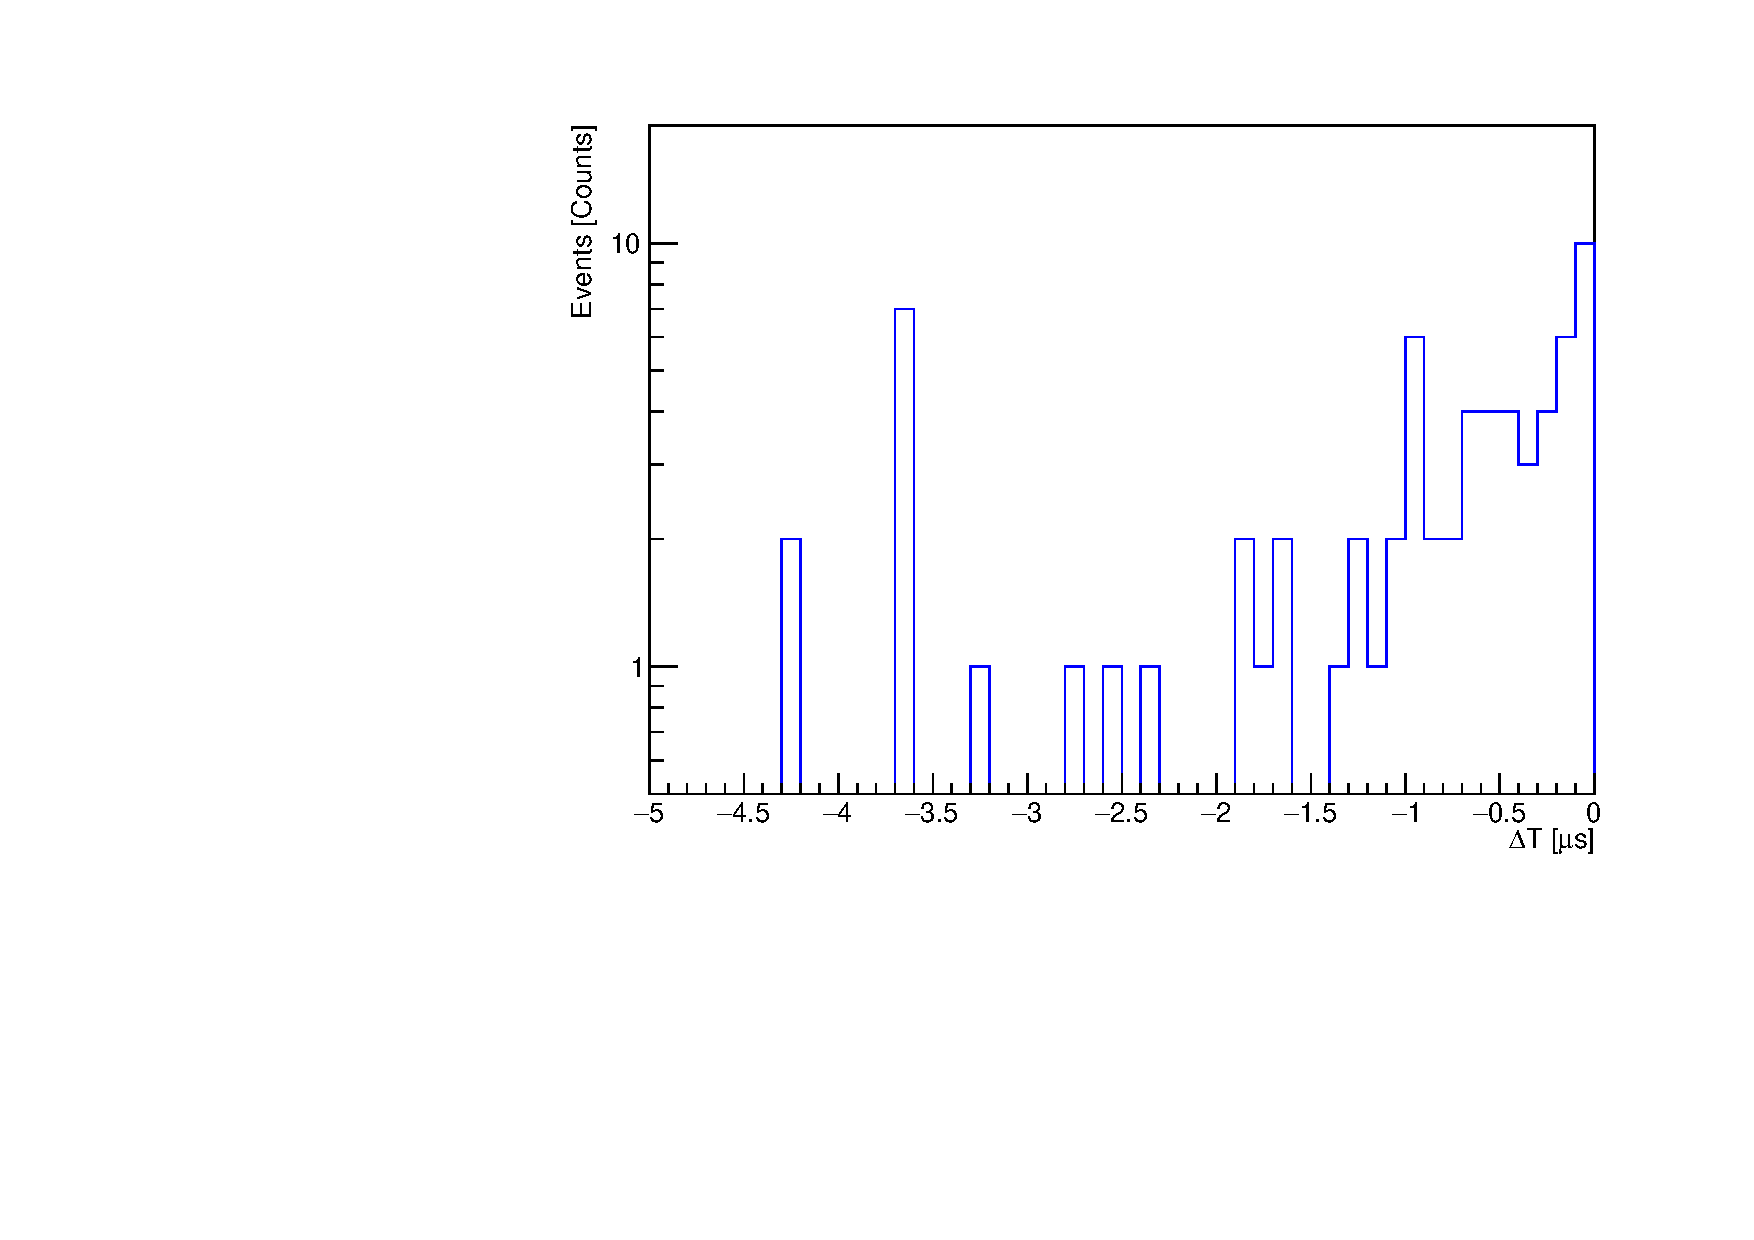
\includegraphics[width=100mm]{./Bilder/TriggerTimeOnly4.pdf}
	\fi%
	\caption{
	    Counts plotted over the time difference between the germanium detector event and the signal in the photomultipliers.
	    The range of the plot only shows the negative time difference from -5 to 0 $\mu$s.
	    This means that all events creating this plot measured a photomultiplier signal before an germanium detector signal.
	    Due to \nuc{Rb}{85m}'s half life of 1.015$\mu$s an exponential increase should be identifiable but with the low amount of counts no statement can be made. 
	}
    	\label{fig:Trigger4}
\end{figure}

Applying these two restrictions to the LAr veto filtered events and using from those only those photomultiplier events with a signal strength of at least 0.5 phe results in a distribution as shown in figure \ref{fig:Trigger4}.
Only the signals that have measured at least 0.5 phe are of interest because they had the necessary intensity to trigger the LAr veto. 
The x axis is the time difference of the events in the photomultipliers from the signal measured in one of the Germanium detectors.
Theoretically it should be possible to see a exponential increase from the negative scale towards a vanishing time difference.
But due to the small number of events, it is basically impossible to make any statements about the course of these events.
\\

Nevertheless, the number of events of interest was reduced from 1728 to only 55.  
These remaining events can now be manually examined with a software called GerLa.
This tool allows one to search for a specific events and see all recorded signals of the Germanium detectors and the photomultipliers around the time frame of this event.
\\

With this program one can now perform a manual filter.
This can be done by looking at the remaining 55 events individually and decide whether to reject an event or not using a specific protocol.
This protocol consists of rejecting every event that has a combined light intensity of over 5 phe and every event that only has a negative time difference in a signal weaker than 0.5 phe.
The upper limit of the light intensity originates again from the expected number of photons as described earlier.
\\

\begin{figure}[t!]
	\centering
	\ifmakefigures%
	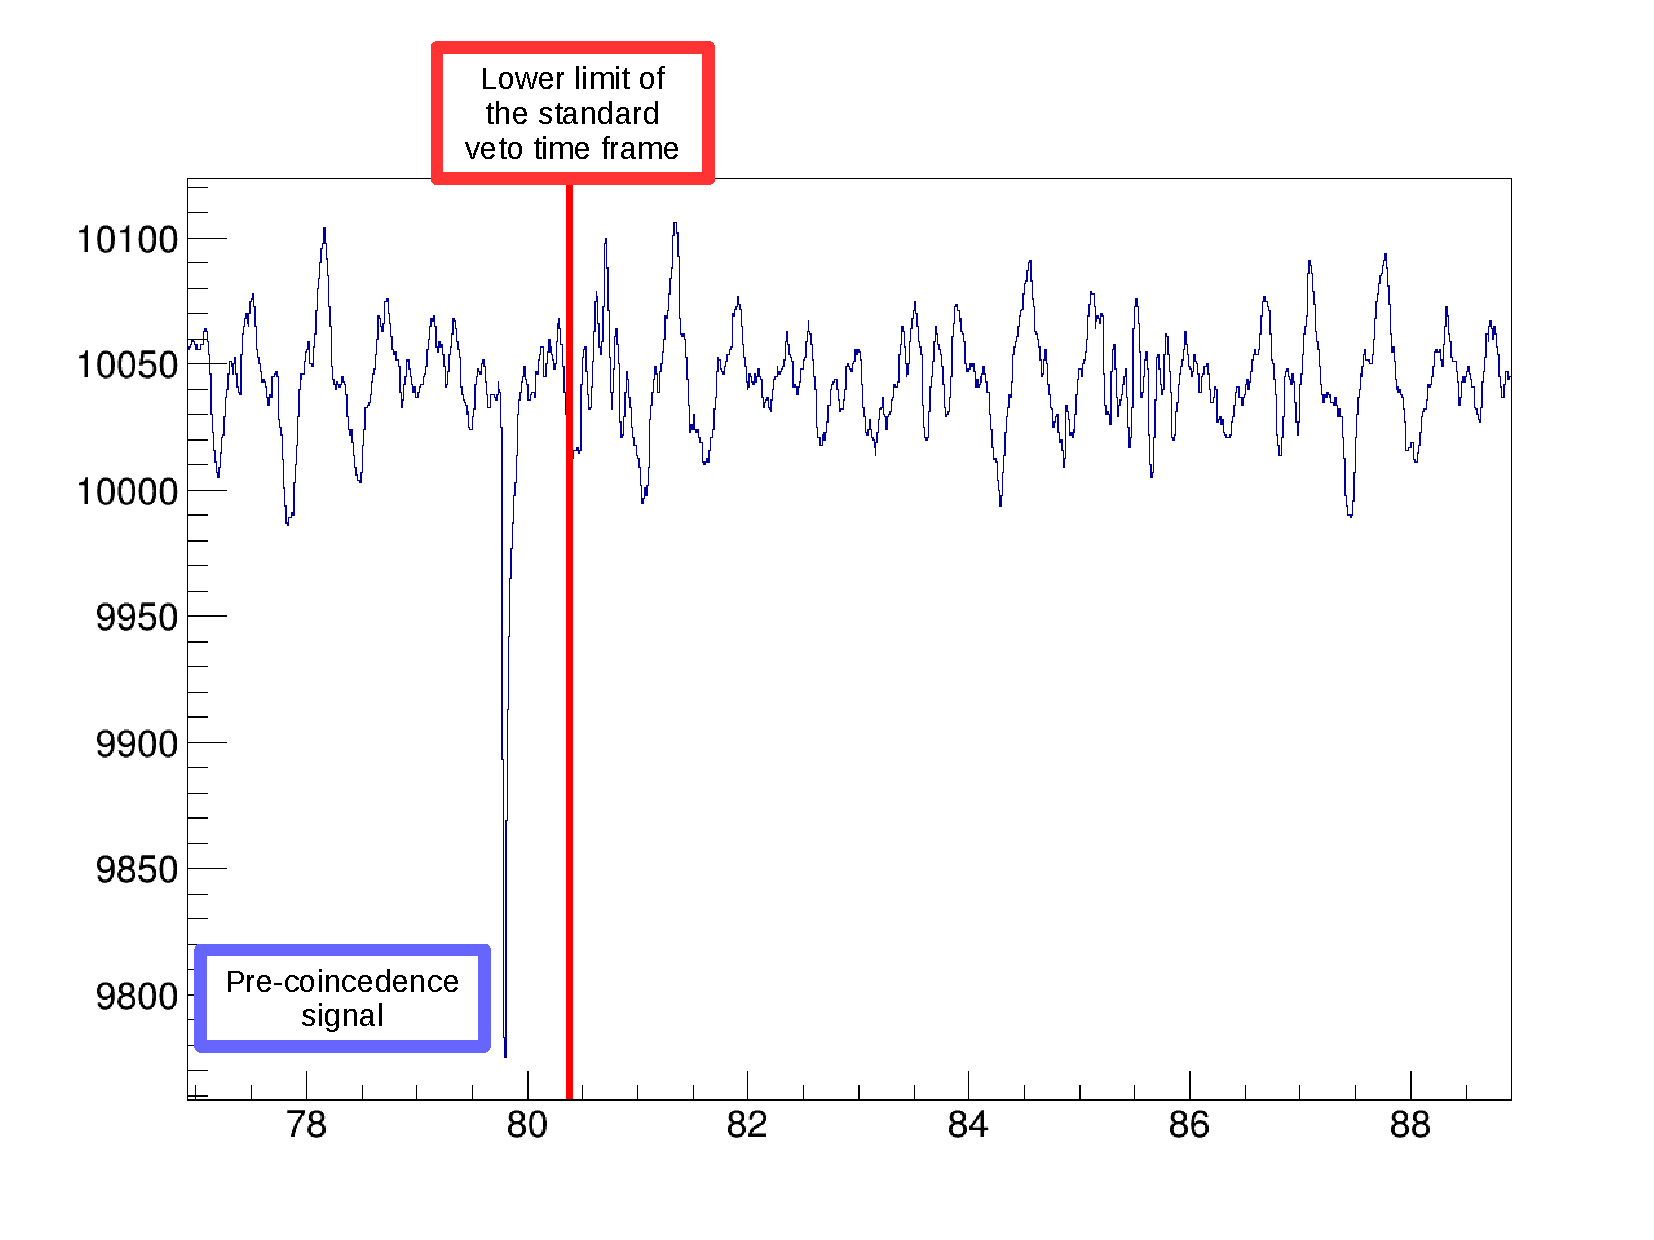
\includegraphics[width=100mm]{./Bilder/BeispielSignal.pdf}
	\fi%

	\caption{
    The recorded signal of photomultiplier tube P4 in event 1614036. 
    In it is the raw energy signal plotted over the recorded time frame. 
    The blue line indicates the moment in time in which an event in one of the germanium detectors was measured. 
    From it one can see that the photomultiplier signal occurred before the germanium detector signal.   
    }
    	\label{fig:BeispielSignal}
\end{figure}

While going through each of the 55 events, it quickly was realized that this procedure does not work as well as we hoped it would.
From the remaining 55 only a handful of events were unambiguous enough that one can claim that the photons must originate from expected beta electron.
After this much filtering it can assume the few that were found are probably all in fact caused by a \Kr\ decays.
Signals like the one shown in figure \ref{fig:BeispielSignal} are a rare example of an almost model signal that were expected to be measured.
The great majority of other events were either background events in the SiPM that seem to randomly triggered the LAr veto or the combined signal strength was much higher than 5 phe.\\

This leads to the conclusion that the majority of signals in the photomultiplier with a negative time difference were in fact not caused by the beta electrons scintillation light but rather coincidences with other signals.
This means it is practically impossible to recover any of them with the process presented here.

The recovery attempt has failed.
\\

Nevertheless we are still able to make some qualitative estimations about why approach might not have worked. 
The problem of this recovery attempt seems to be that the majority of events detected with a negative time difference are in fact background events.
This conclusion came from the fact that almost none of the events investigated have shown the features we expected from them.

An indicator for this can be seen in the fact that the majority of light signals have been measured in the PMTs.
As it will be shown in section \ref{sec:MonteCarlo514}, basically all of the decays that created a measurable 514keV event have happened in the vicinity of the detectors.
The detectors themselves should already block some of the light but when a photon is detected in a photomultiplier it would most likely be a SiPM.
This is because the nylon fibers surrounding the germanium detectors are more likely to absorb and guide the scintillation light to the SiPM than a photon to reach a PMT above or below the detector arrays.
Now that the majority of the detected light events are measured in the PMTs it is very unlikely that these are caused by a \Kr\ decay.

%That the majority of the 
%This might also be able to be seen from figure \ref{fig:AntiLArBEGes} and \ref{fig:AntiLArCOAX}.
%From them one was able to see that the LAr veto also filtered out some of the 514keV line events.
%But from it can also be seen, that the ratio of events filtered out at the 514keV mark over the non filtered value [$N_{\unit{vetoed}}(514\unit{keV})/N_{\unit{unfilered}}(514\unit{keV})]$ is of about the same size as in the background area whereas the positron electron peak shows much higher ratio.
%Considering this the peaks in \ref{fig:AntiLArBEGes} and \ref{fig:AntiLArCOAX} probably came to be  due to the same relative amount of events have their liquid argon veto triggered because of background events.
Because of this it is rather questionable whether the LAr veto is even a good identifier to use when it also filters out events in which background can trigger the veto.
A satisfactory answer however will only be able to obtain through a quantitative analysis which will be performed in the following chapter.
\\
